Due to the lifetime ($c\tau > 2$ mm) and mass ($m > 10$ GeV) requirements applied at vertex selection, no SM background is expected in the signal region in search for displaced dilepton resonance. Therefore, two non-collision backgrounds and background from low-mass vertices are considered in this search. In Section~\ref{sec:random_crossing}, background from \textit{random-crossing} of two uncorrelated tracks are estimated. The cosmic ray background is estimated in Section~\ref{sec:cosmic_ray}, and the low-mass background which results from low-mass vertices is estimated in Section~\ref{sec:low_mass}

\subsection{Random-crossing background}
\label{sec:random_crossing}
%High luminosity in 2016 data ($\langle\mu\rangle\approx 24.9$) %where $<\mu>$ is average number of interactions per bunch crossing, made 
%The random-crossing of two uncorrelated tracks is one of the dominant source of background in search for displaced dilepton vertices due to increasing pileup in Run 2 with $\langle\mu\rangle\approx 24.9$ in 2016 data. 
The random-crossing of two uncorrelated tracks is a major source of the backgrounds in the search for displaced dilepton vertices. This background is expected to increase with more pile up in Run 2.

This random-crossing background is estimated by the \textit{track flipping} method in which secondary vertex reconstruction is performed on each pair of tracks from all possible combinations of tracks after one random track from each pair is flipped with respect to the primary vertex. Because one track is flipped in each pair of tracks, the resulting vertices provide good estimation for random-crossing background.

The track flipping method is tested on the background MC samples. As an additional check, the vertices found from this method are compared with vertices found from another random-crossing background estimation method, the \textit{event mixing}. In Section~\ref{sec:random_crossing_data}, the random-crossing background are estimated using the track flipping method with 32.8 $\mathrm{fb^{-1}}$ of 2016 data sample, and its systematic uncertainties are estimated in Section~\ref{sec:random_crossing_systematics}.

\subsubsection{MC study}
\label{sec:random_crossing_MC}
The track flipping method is tested using the background MC sample with 2.4 M events as described in Section~\ref{sec:data_MC}. Events are selected by the same requirement described in Section~\ref{sec:signal_efficiency}. From the selected events, tracks identified as muon, electron, or neither, referred as muon, electron, or non-leptonic track, respectively, are selected with the track criteria (Table~\ref{table:vertex_track_selection_simple}) as in the secondary vertexing algorithm for consistency. Leptons are required to pass the same selection criteria described in Table~\ref{table:lepton_requirement}. Non-leptonic tracks are required to pass the minimal kinematic selection ($p_{T} > 10 GeV, \eta < 2.5$ to match with the kinematic selection for leptons.

Track pairs are created from all possible combination of muon, electron, or non-leptonic tracks which fall into one of the six categories, $\mu\mu$, $ee$, $e\mu$, $e$x, $\mu$x, or xx track pair, where $x$ represents a non-leptonic track. For each pair of tracks, one track is randomly flipped with respect to the beam spot ($d_{0}\rightarrow -d_{0}, z_{0}\rightarrow -z_{0}, \phi\rightarrow\phi-\pi, \theta\rightarrow\pi-\theta$). The flipped track and the other track in the pair are used to estimate the background from uncorrelated tracks.

%Two tracks from each pair after flipping one track become uncorrelated.

The same secondary vertex algorithm used in the reconstruction of data or MC sample is performed on the track pairs with one track flipped to reconstruct secondary vertices. Vertex selection cuts similar to the cuts listed in Table~\ref{table:vertex_track_selection_simple} are applied to the vertices found by the track flipping. The only differences in the vertex cuts are:
\begin{itemize}
\item Trigger matching is only required for $\mu\mu$, $ee$, and $e\mu$ vertices because non-leptonic tracks cannot be matched to lepton triggers, 
\item Filter matching is only required for $\mu\mu$, $ee$, and $e\mu$ vertices for the same reason.
\end{itemize}

Because trigger and filter matchings are not required in the control and validation region, the track flipping method provides conservative background estimation. Figure~\ref{fig:m_FBE_cutflow_MC} shows the vertex cut flow applied on xx vertices from the background MC samples.

%\begin{figure}[!htb]
\begin{figure}[tb]
	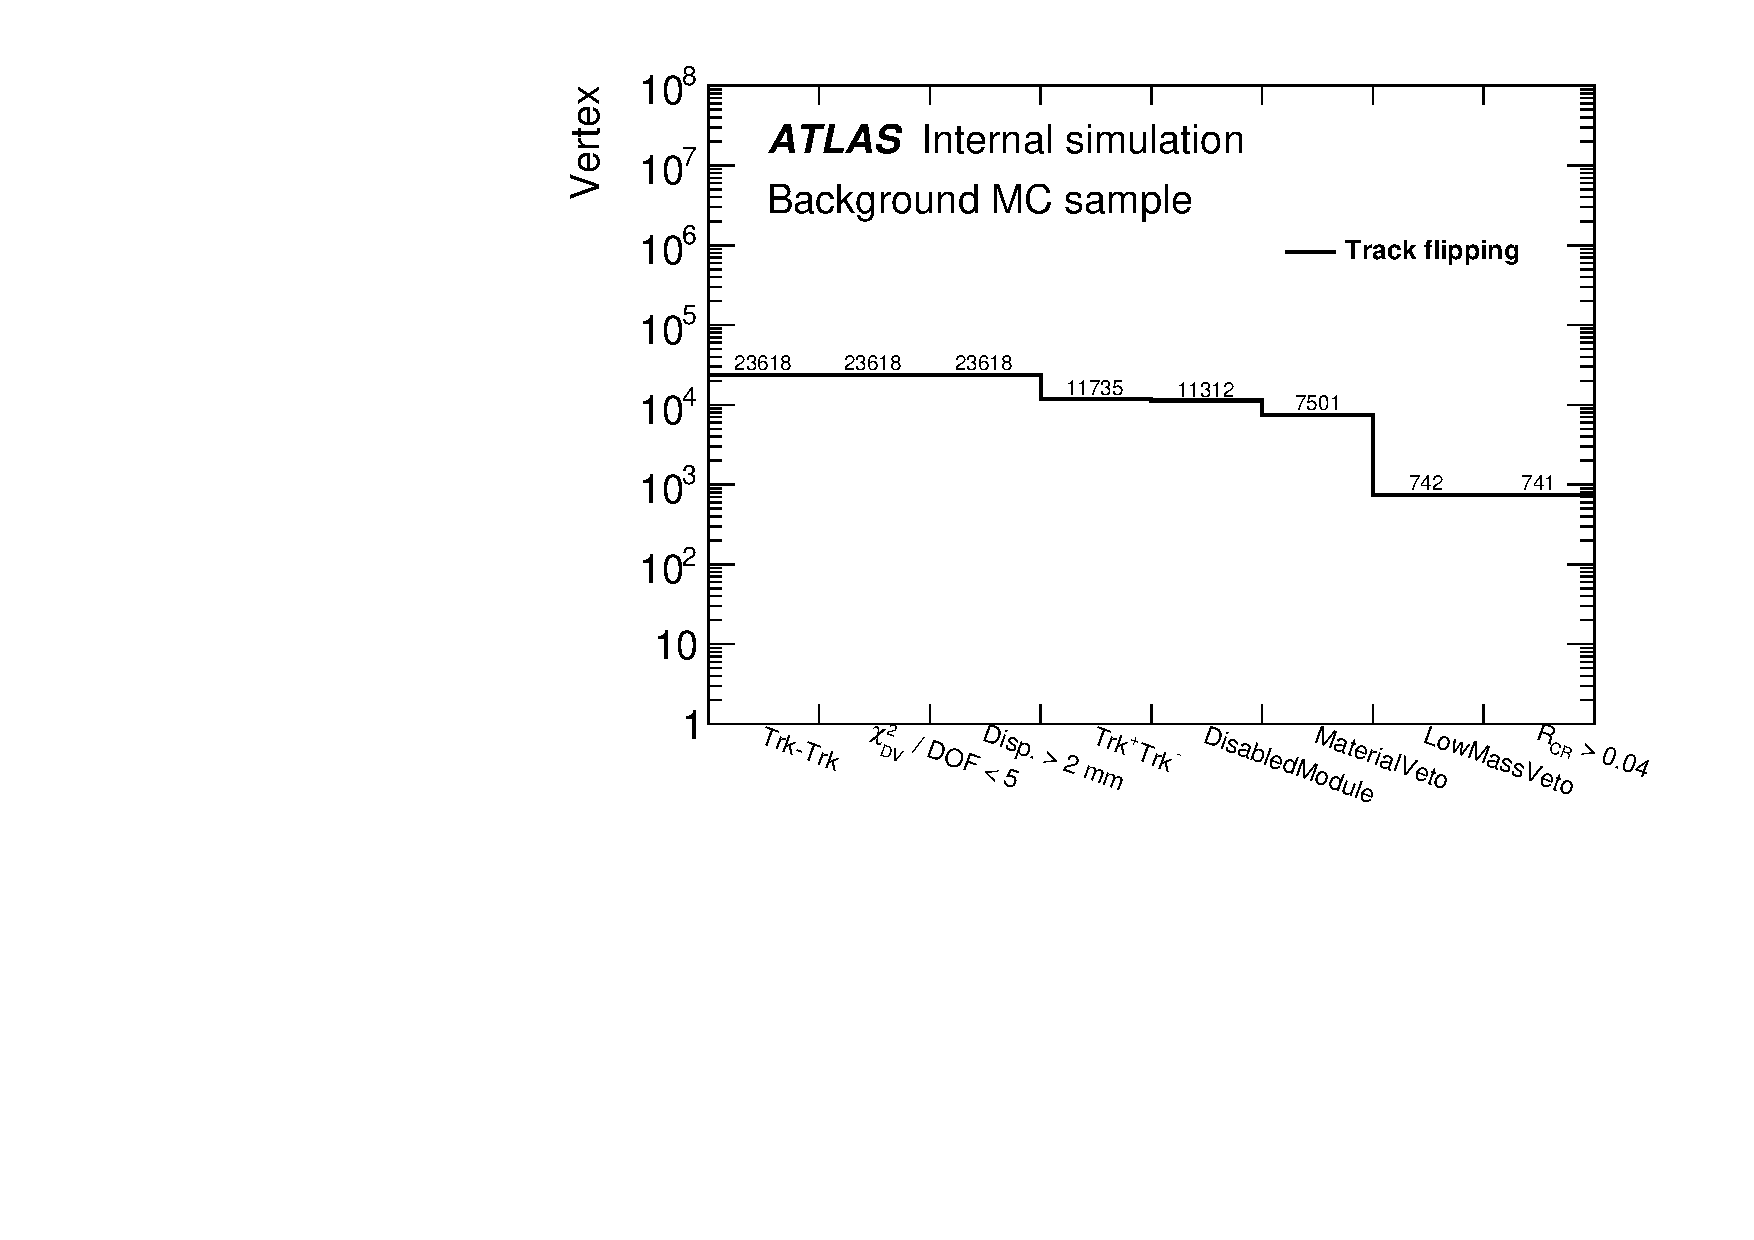
\includegraphics[width=0.60\textwidth]{figures/m_FBE_cutflow_MC.pdf}
	\centering
	\caption{Vertex cut flow applied on xx vertices from the track flipping method}
	\label{fig:m_FBE_cutflow_MC}
\end{figure}

The resulting vertices, referred as track-flipping vertices, are compared with the vertices reconstructed by the reconstruction described in Section~\ref{sec:track_vertex_reconstruction} in the MC samples. The same event selection and the vertex selection described in Section~\ref{sec:signal_efficiency} are applied to the vertices in the data sample. Because of minimum invariant mass ($m > 10$ GeV), minimum displacement ($r_{DV} > 2$ mm), and cosmic veto ($R_{\mathrm{CR}} > 0.01$) cuts, the reconstructed vertices in the MC sample are expected to be purely from random-crossing.

In addition, the track-flipping are compared with another random-crossing background estimation method, the \textit{event mixing}. In this method, tracks are sampled from data or MC sample, and the probability, denoted by $p_{\mathrm{rc}}$, for a pair of tracks to form a vertex by random-crossing is estimated by randomly mixing tracks from different events. Using $p_{\mathrm{rc}}$ and the total number of pairs of tracks in data or MC sample, random-crossing background is estimated. The details on this method can be found in []. The same event, track, and vertex selections are applied for consistency with the track flipping.

The xx vertices found from the track flipping, reconstructed in the MC sample, and the estimation from the \textit{event mixing} are compared in Table~\ref{table:random_vertex_count}. No $\mu\mu$, $ee$, or $e\mu$ vertices was found or expected from these methods.
 
\begin{table}[!htb]
  \centering
  \begin{tabular}{ c  c c c }
    \hline
    \hline
	Vertex Type					&Track flipping	&\textit{Event Mixing}	& Background MC Samples \\
    \hline
	$\mu$x						&	1						&	1.3 				&	0					\\
	$e$x						&	0						&	0.3 				&	0					\\
	xx						&	741 					&	714.0				&	676 				\\
    \hline
    \hline
  \end{tabular}
  \caption{Comparison of the number of xx vertices found in the track flipping, estimated from the \textit{event mixing}, and reconstructed in the background MC samples.}
  \label{table:random_vertex_count}
\end{table}

The xx vertex yields from the track flipping and the \textit{event mixing} methods agree within the statistical uncertainty. The xx vertex distributions of the vertices from the track flipping, \textit{event mixing}, and from reconstruction are shown in Figure~\ref{fig:random-crossing_vertex_dist}. The distributions of the track flipping and the \textit{event mixing} agree reasonably well with the distributions of vertices found from the reconstruction.

%, and both methods slightly over-estimated the random-crossing background by $\approx 5.8\%$ in the case of xx vertices.

\begin{figure}[!htb]
    \centering
    \subfloat[]{\label{subfig:random-crossing_M}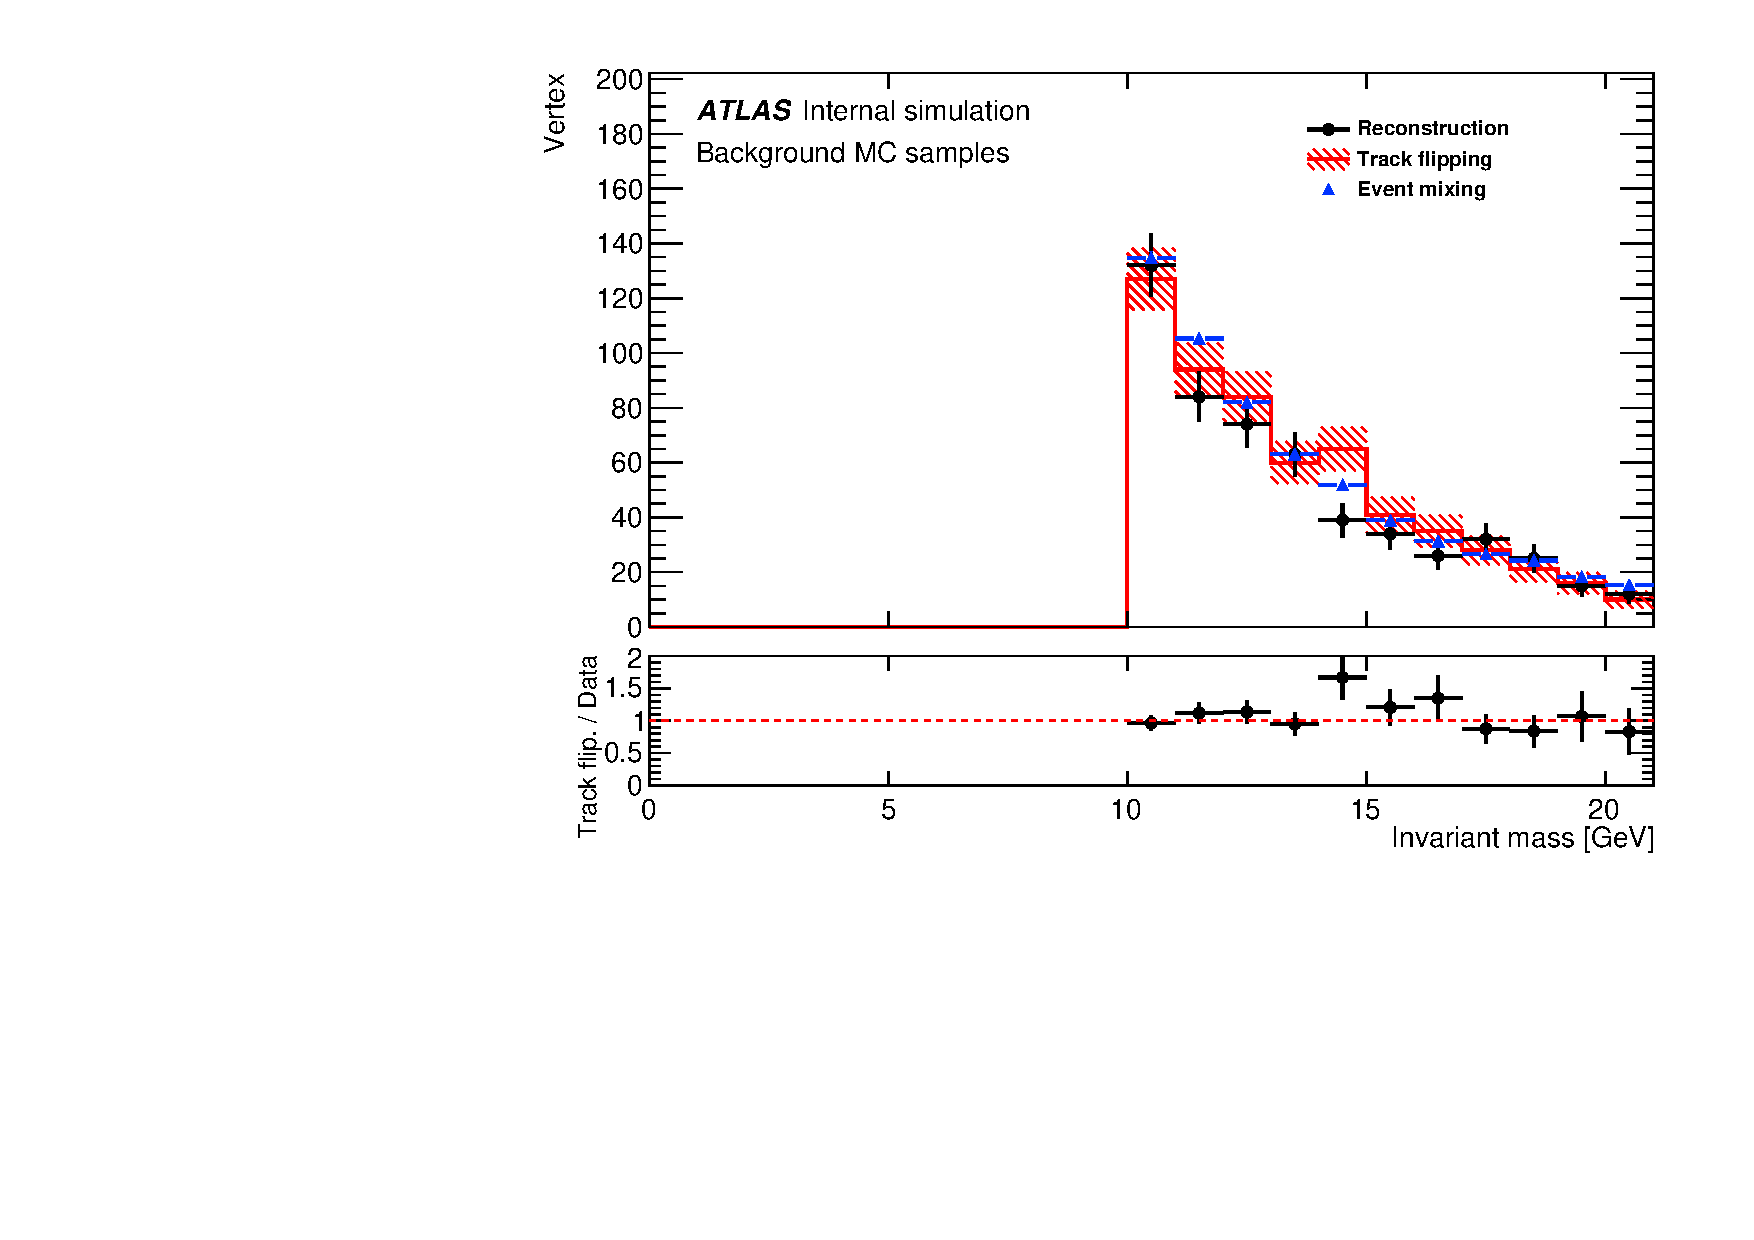
\includegraphics[width=0.45\textwidth]{figures/m_FBE_M.pdf}}
    \subfloat[]{\label{subfig:random-crossing_chi2ndof}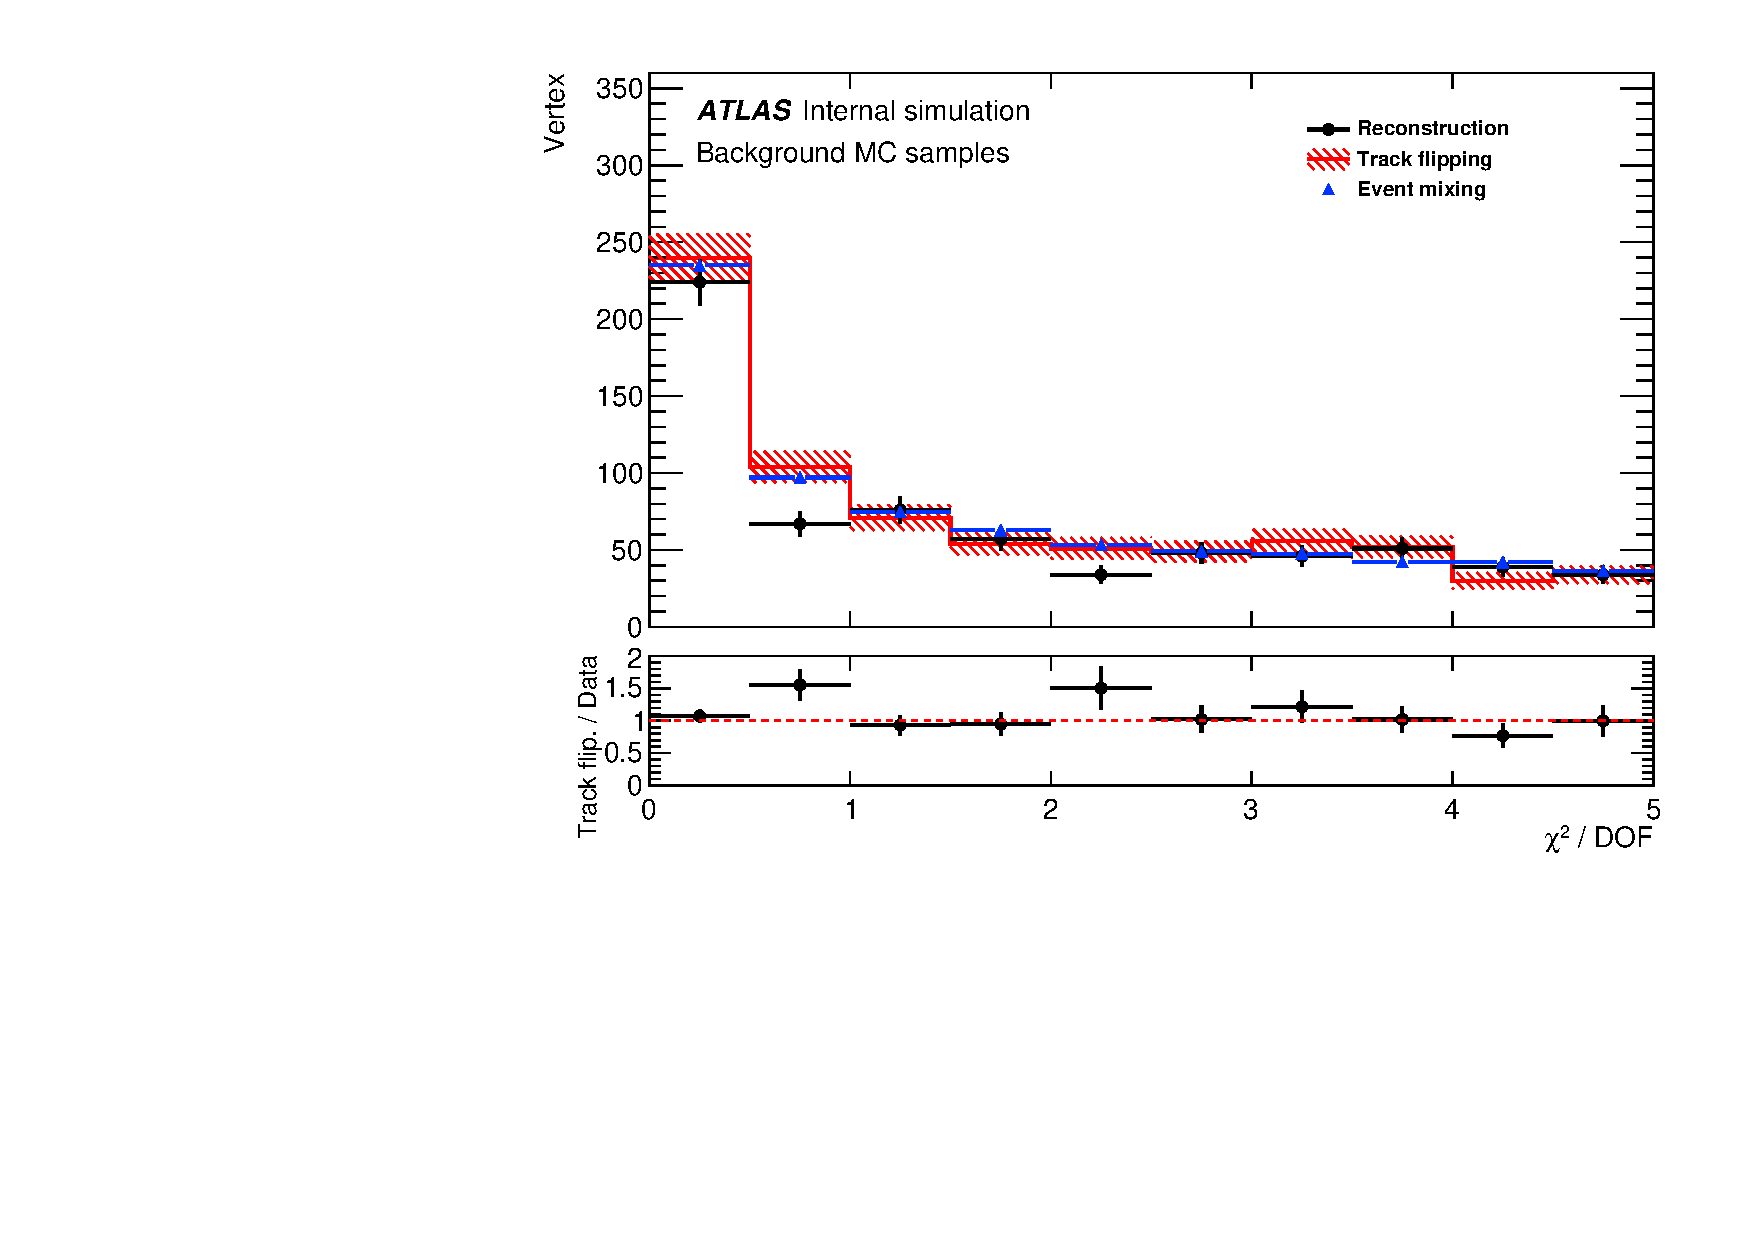
\includegraphics[width=0.45\textwidth]{figures/m_FBE_chi2_ndof.pdf}} \\
    \subfloat[]{\label{subfig:random-crossing_r}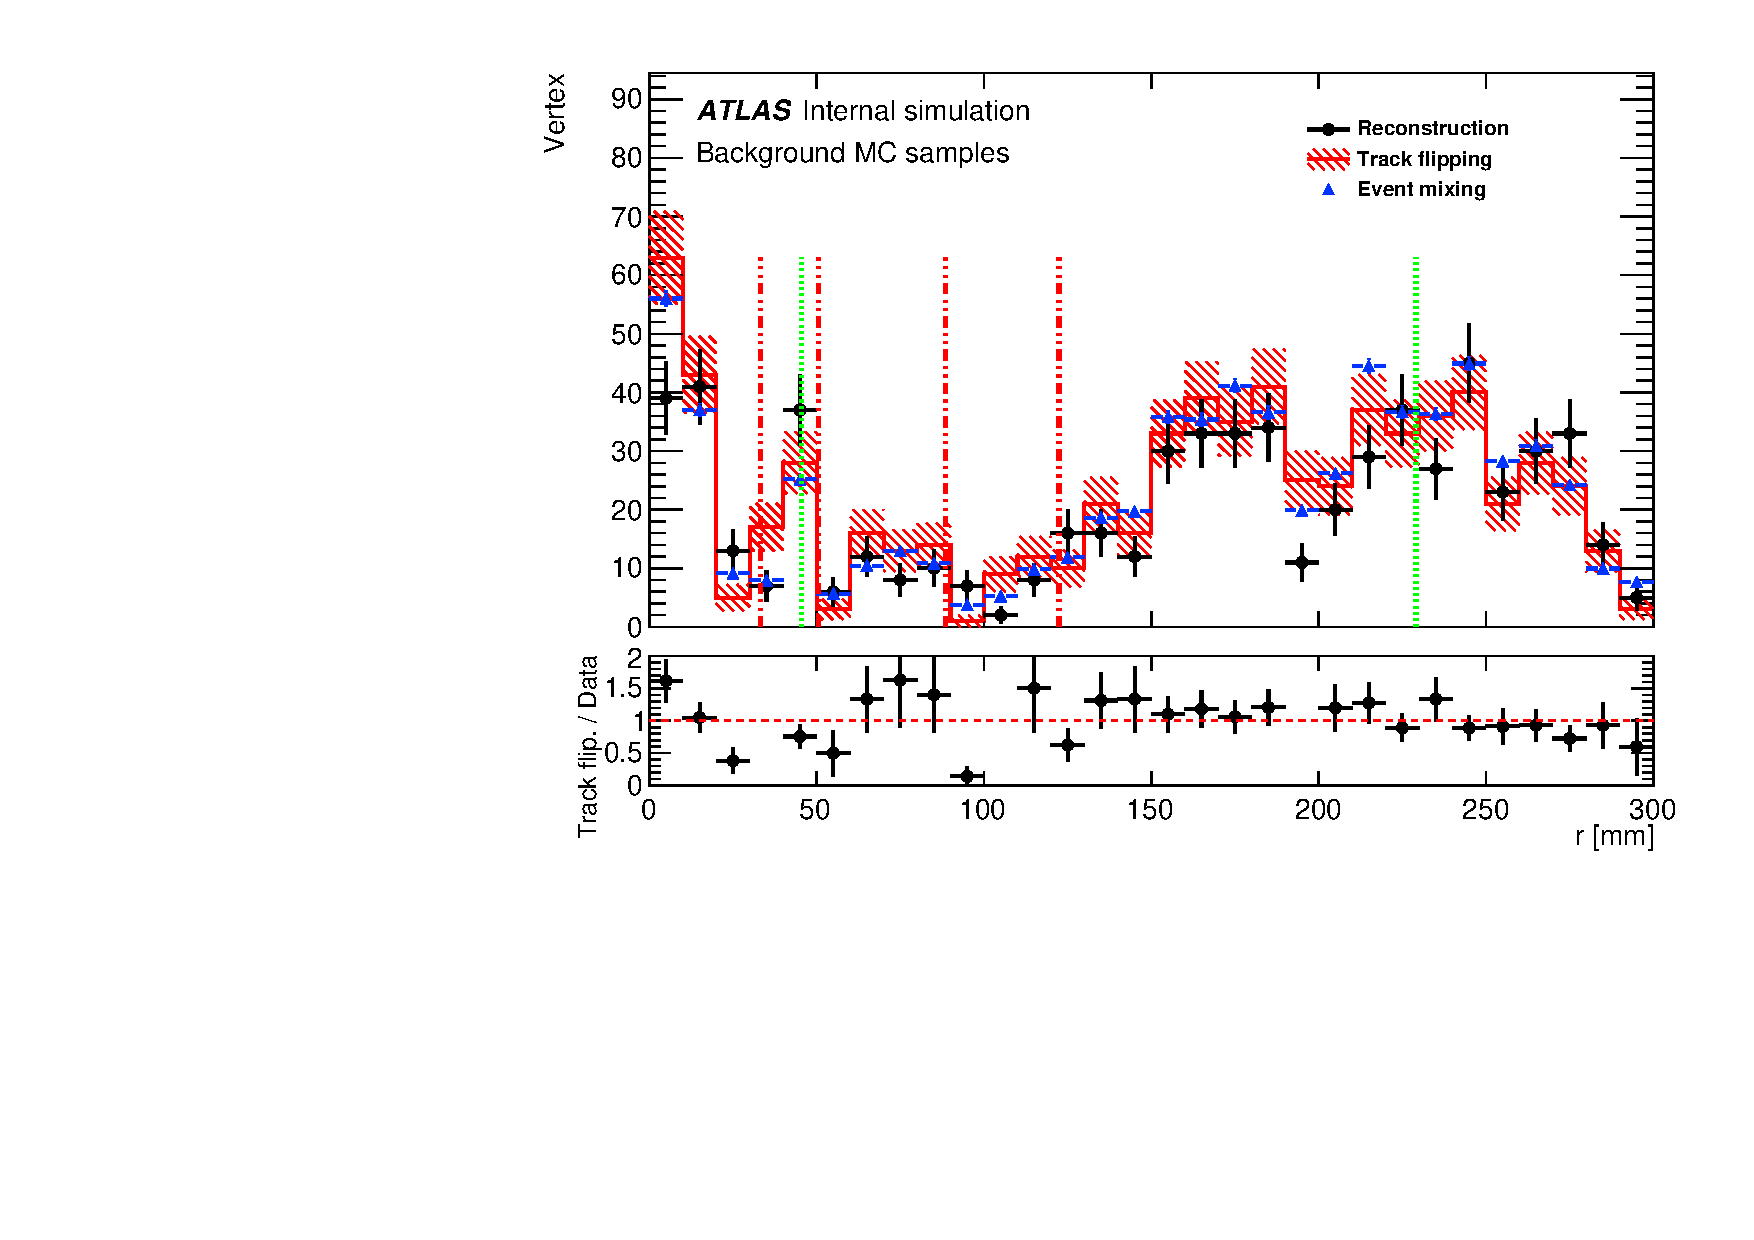
\includegraphics[width=0.45\textwidth]{figures/m_FBE_R.pdf}}
    \subfloat[]{\label{subfig:random-crossing_z}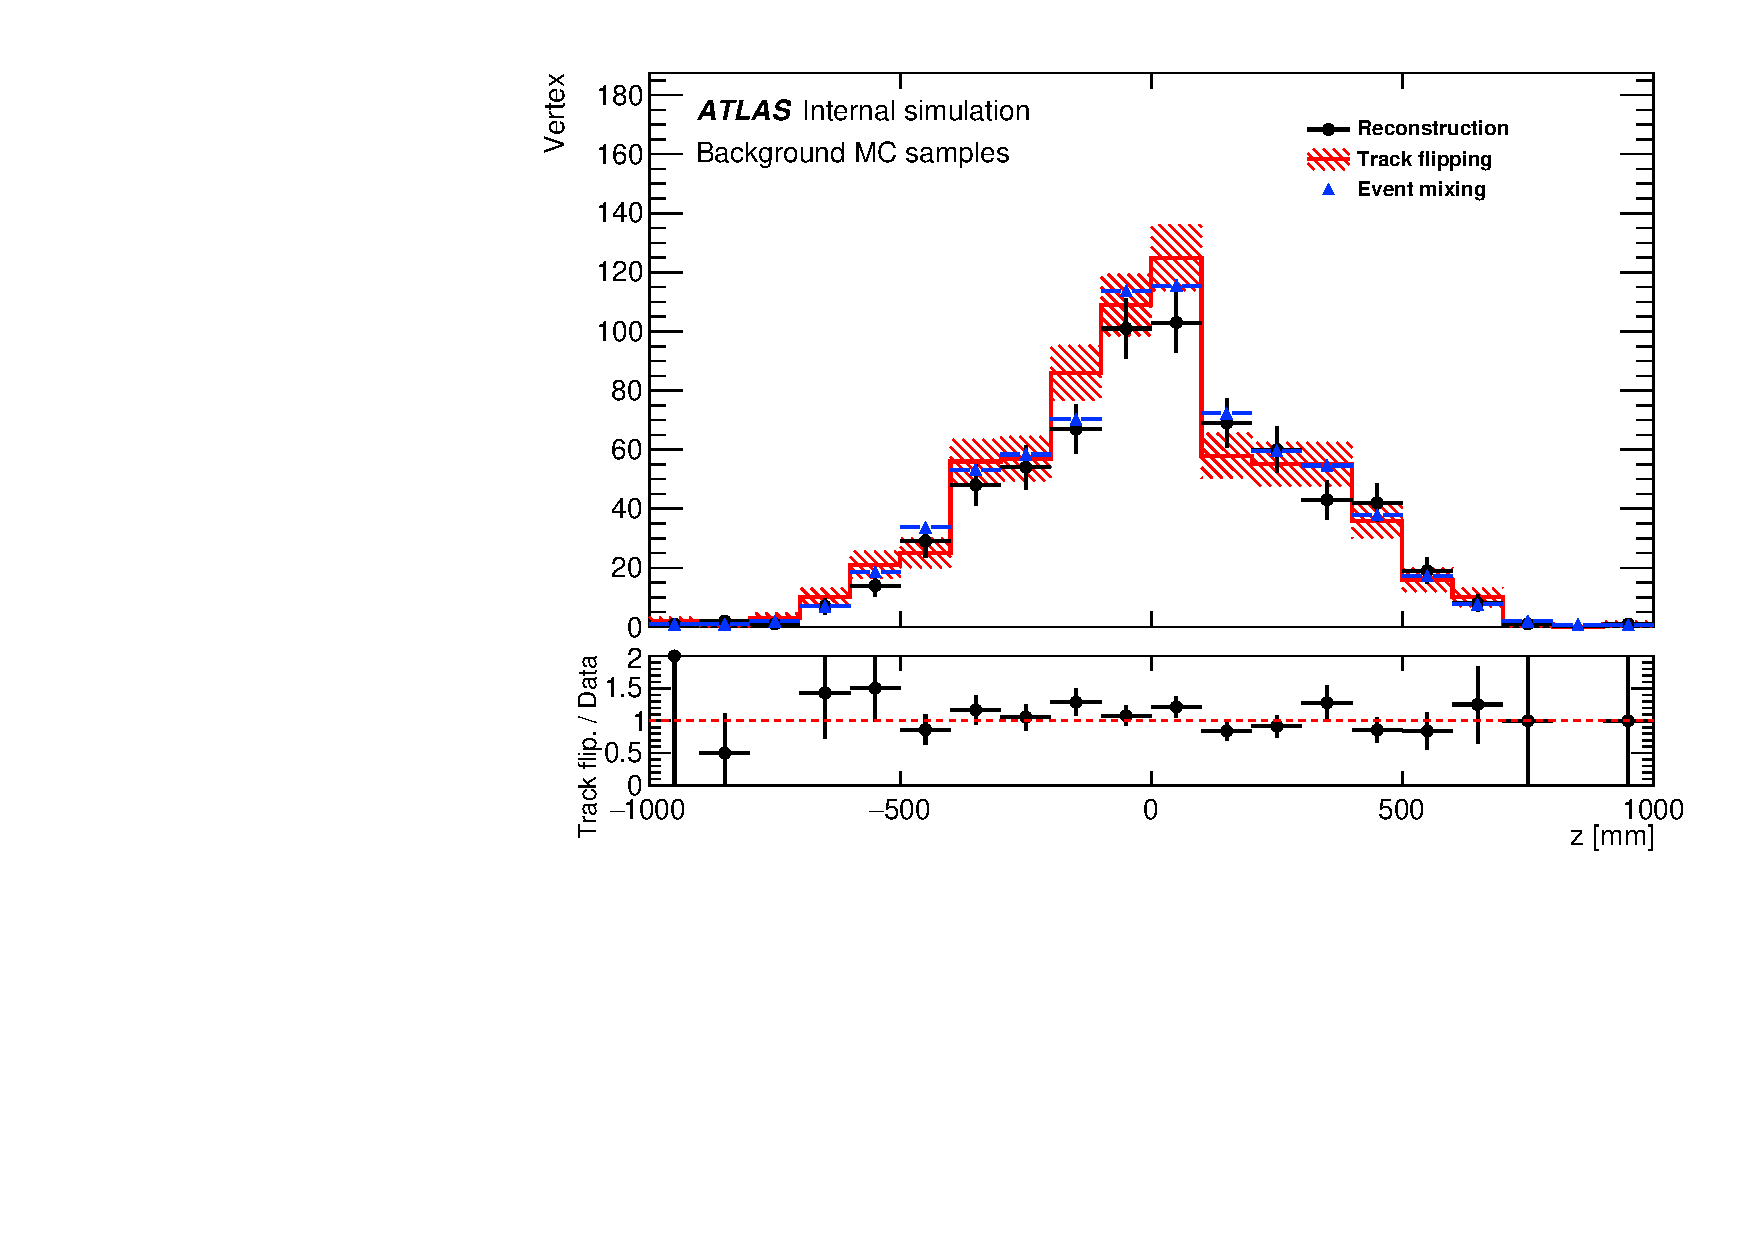
\includegraphics[width=0.45\textwidth]{figures/m_FBE_z.pdf}}
    %\subfloat[l]{\label{subfig:random-crossing_l}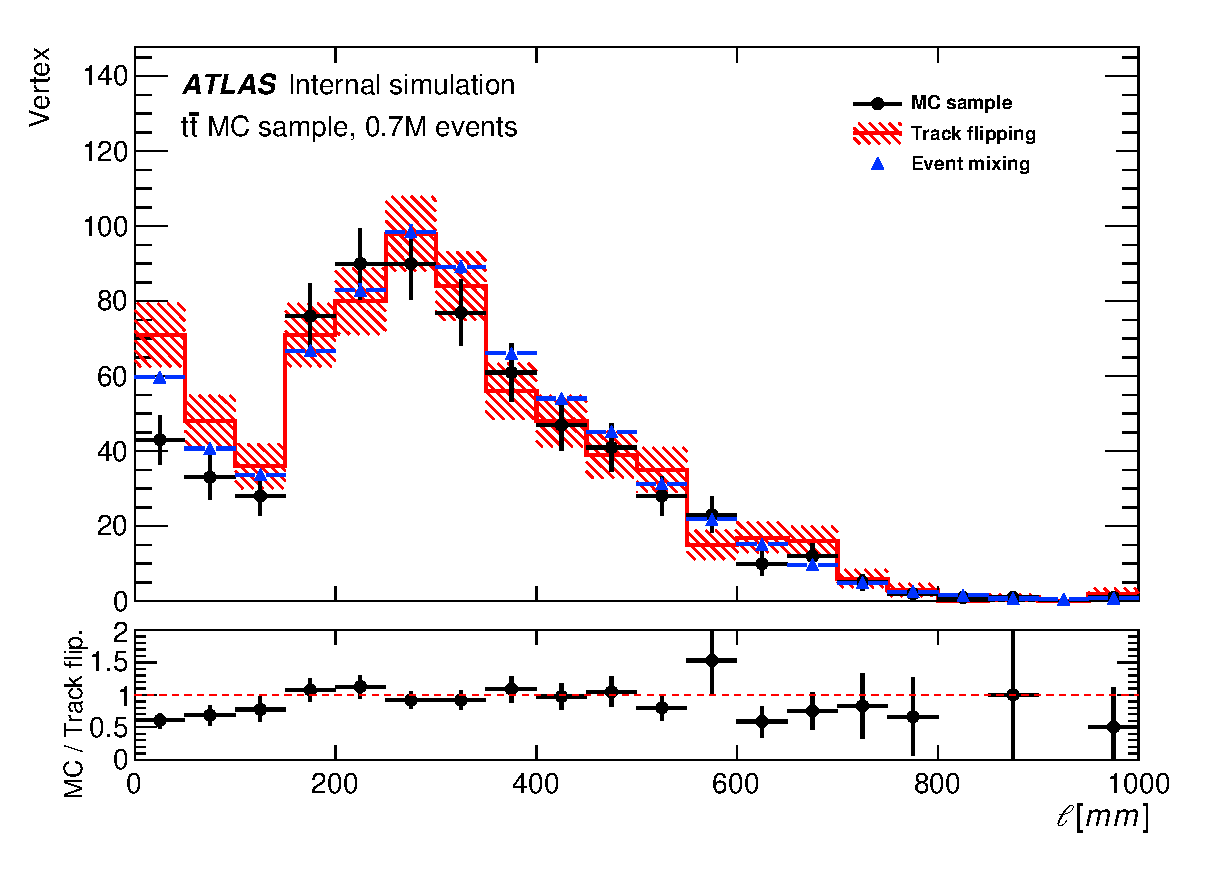
\includegraphics[width=0.45\textwidth]{figures/m_FBE_l.eps}}
    \caption{Comparison of of (a) vertex mass, (b) $\chi^{2} / \mathrm{DOF}$, (c) transverse, and (d) longitudinal position of xx vertices reconstructed, found from the track flipping, and estimated using the \textit{event mixing}. In (c), the red dashed lines indicate the four Pixel layers and the first layer of SCT. The green dotted lines indicate the Inner Support Tube (45.5 mm) and Pixel Support Tube (229 mm).}
    \label{fig:random-crossing_vertex_dist}
\end{figure}

\subsubsection{Estimating random-crossing background with data sample}
\label{sec:random_crossing_data}
Random-crossing background is estimated using 32.8 $\mathrm{fb^{-1}}$ of 2016 data sample described in Section~\ref{sec:data_MC}.

\textbf{Vertex distribution} In control region, the $xx$ vertices found from the track flipping method are compared to the vertices reconstructed in the data sample in Figure~\ref{fig:random-crossing_vertex_dist_data}. The track flipping method reproduces the data reasonably well including some of the structures. 

\begin{figure}[!htb]
    \centering
    \subfloat[]{\label{subfig:random-crossing_M}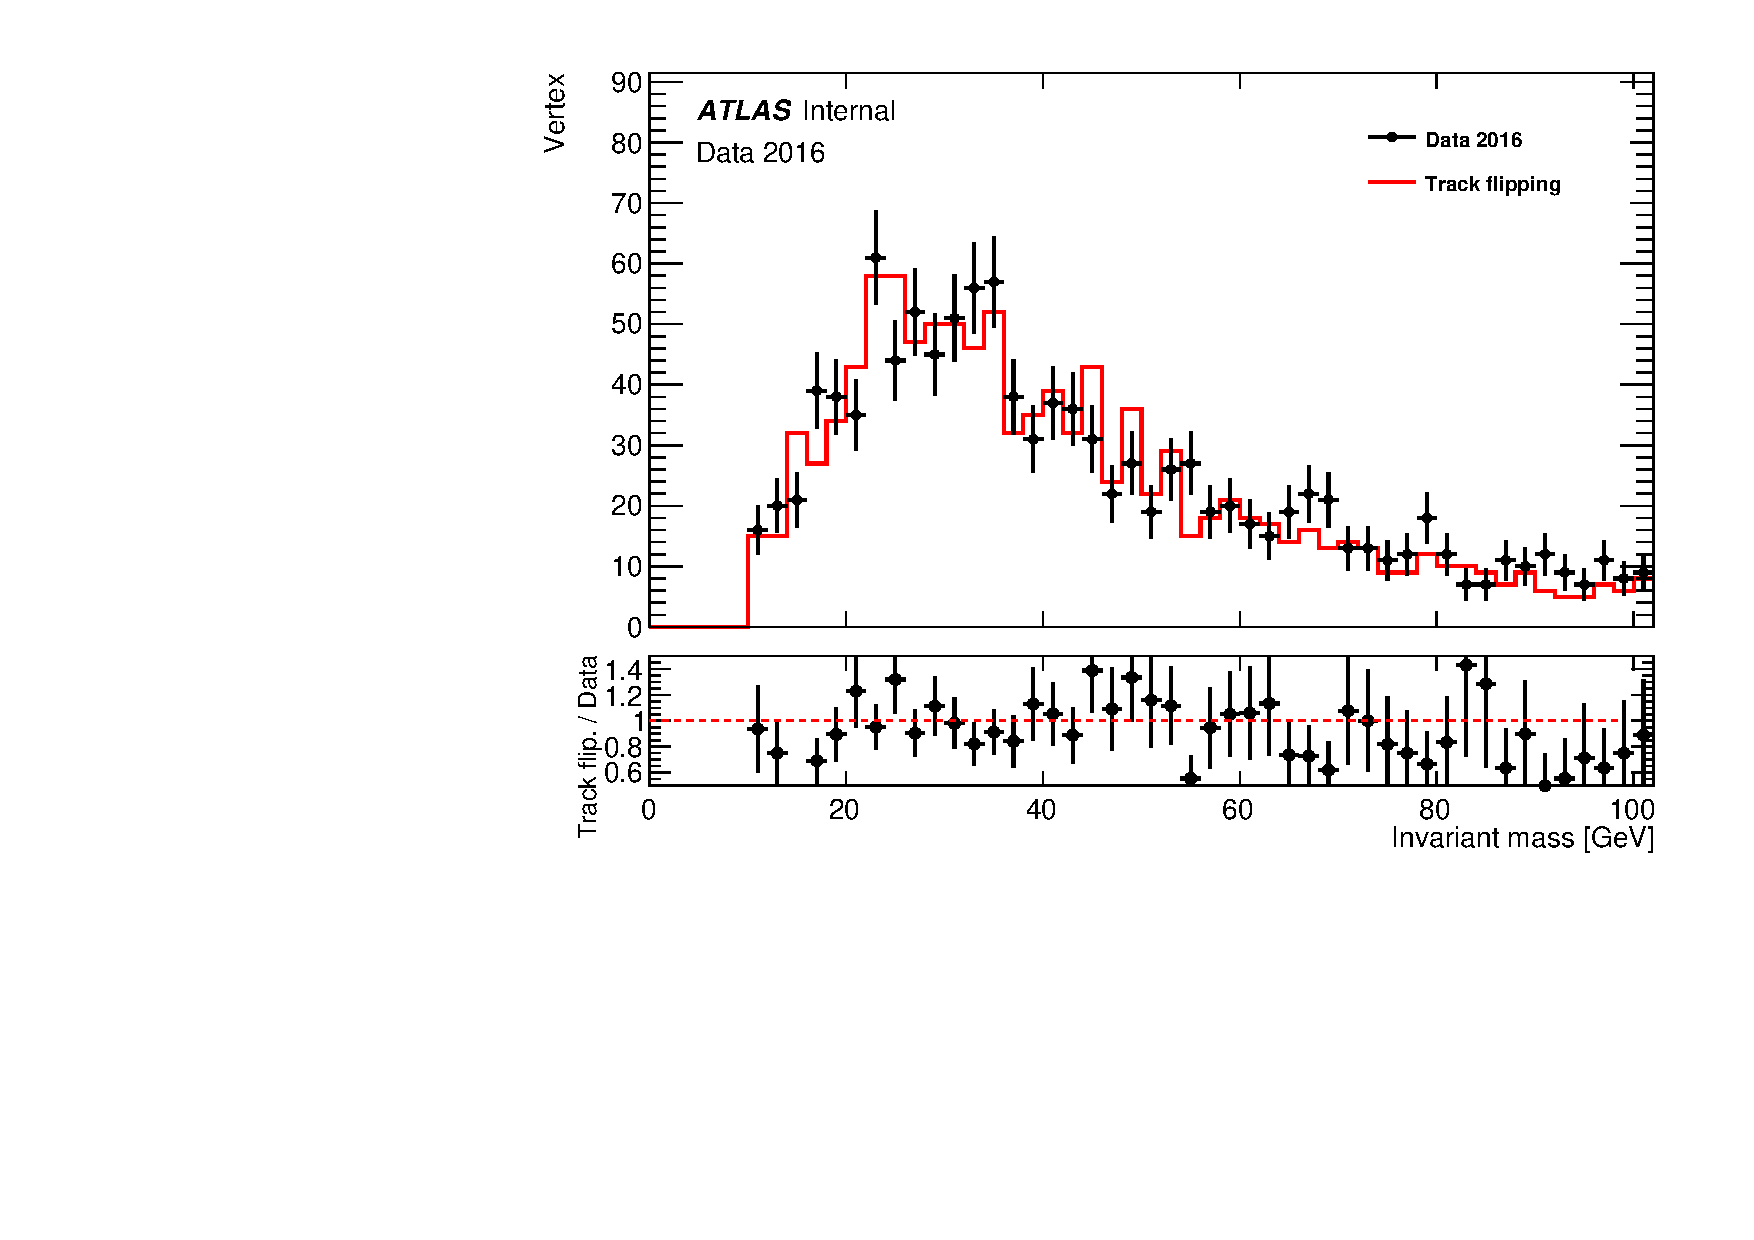
\includegraphics[width=0.45\textwidth]{figures/m_FBE_data_M.pdf}}
    \subfloat[]{\label{subfig:random-crossing_chi2ndof}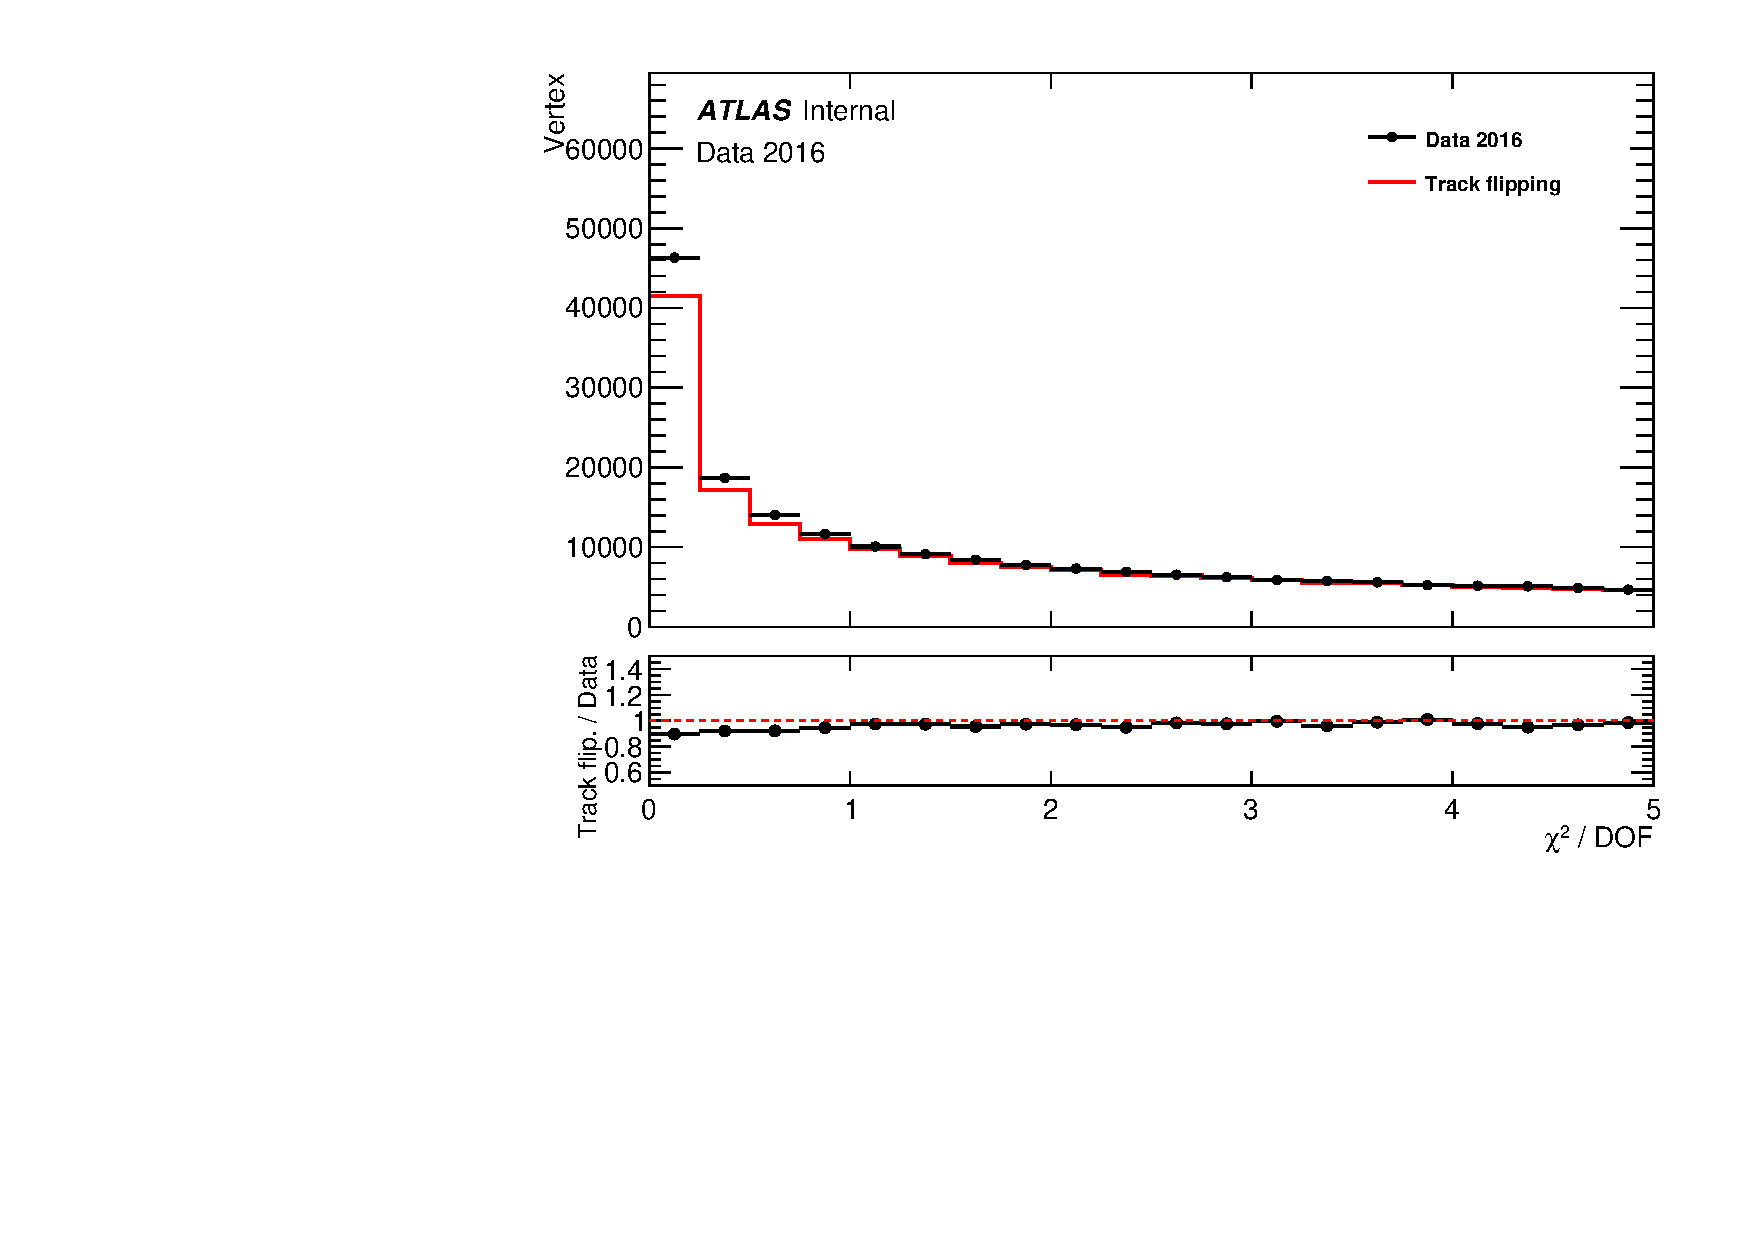
\includegraphics[width=0.45\textwidth]{figures/m_FBE_data_chi2_ndof.pdf}} \\
    \subfloat[]{\label{subfig:random-crossing_r}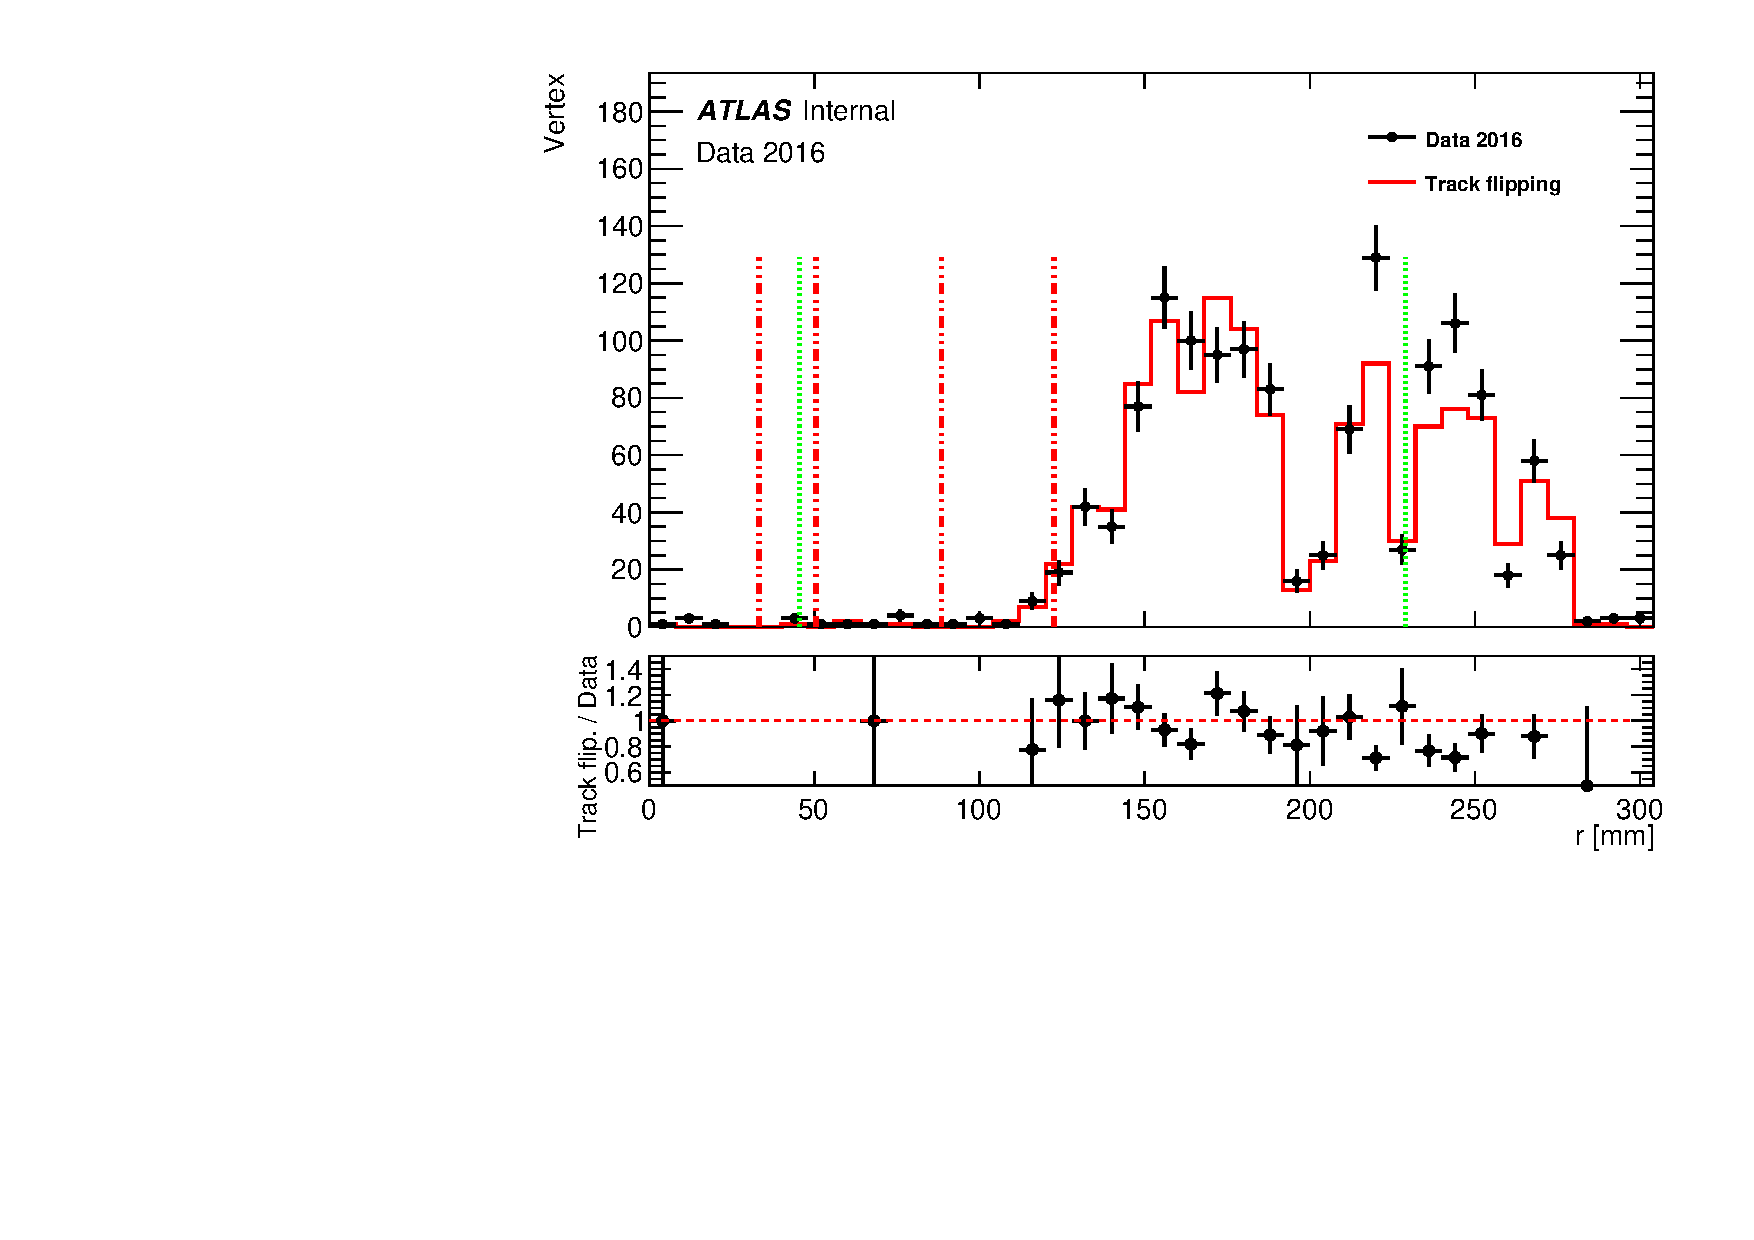
\includegraphics[width=0.45\textwidth]{figures/m_FBE_data_R.pdf}}
    \subfloat[]{\label{subfig:random-crossing_z}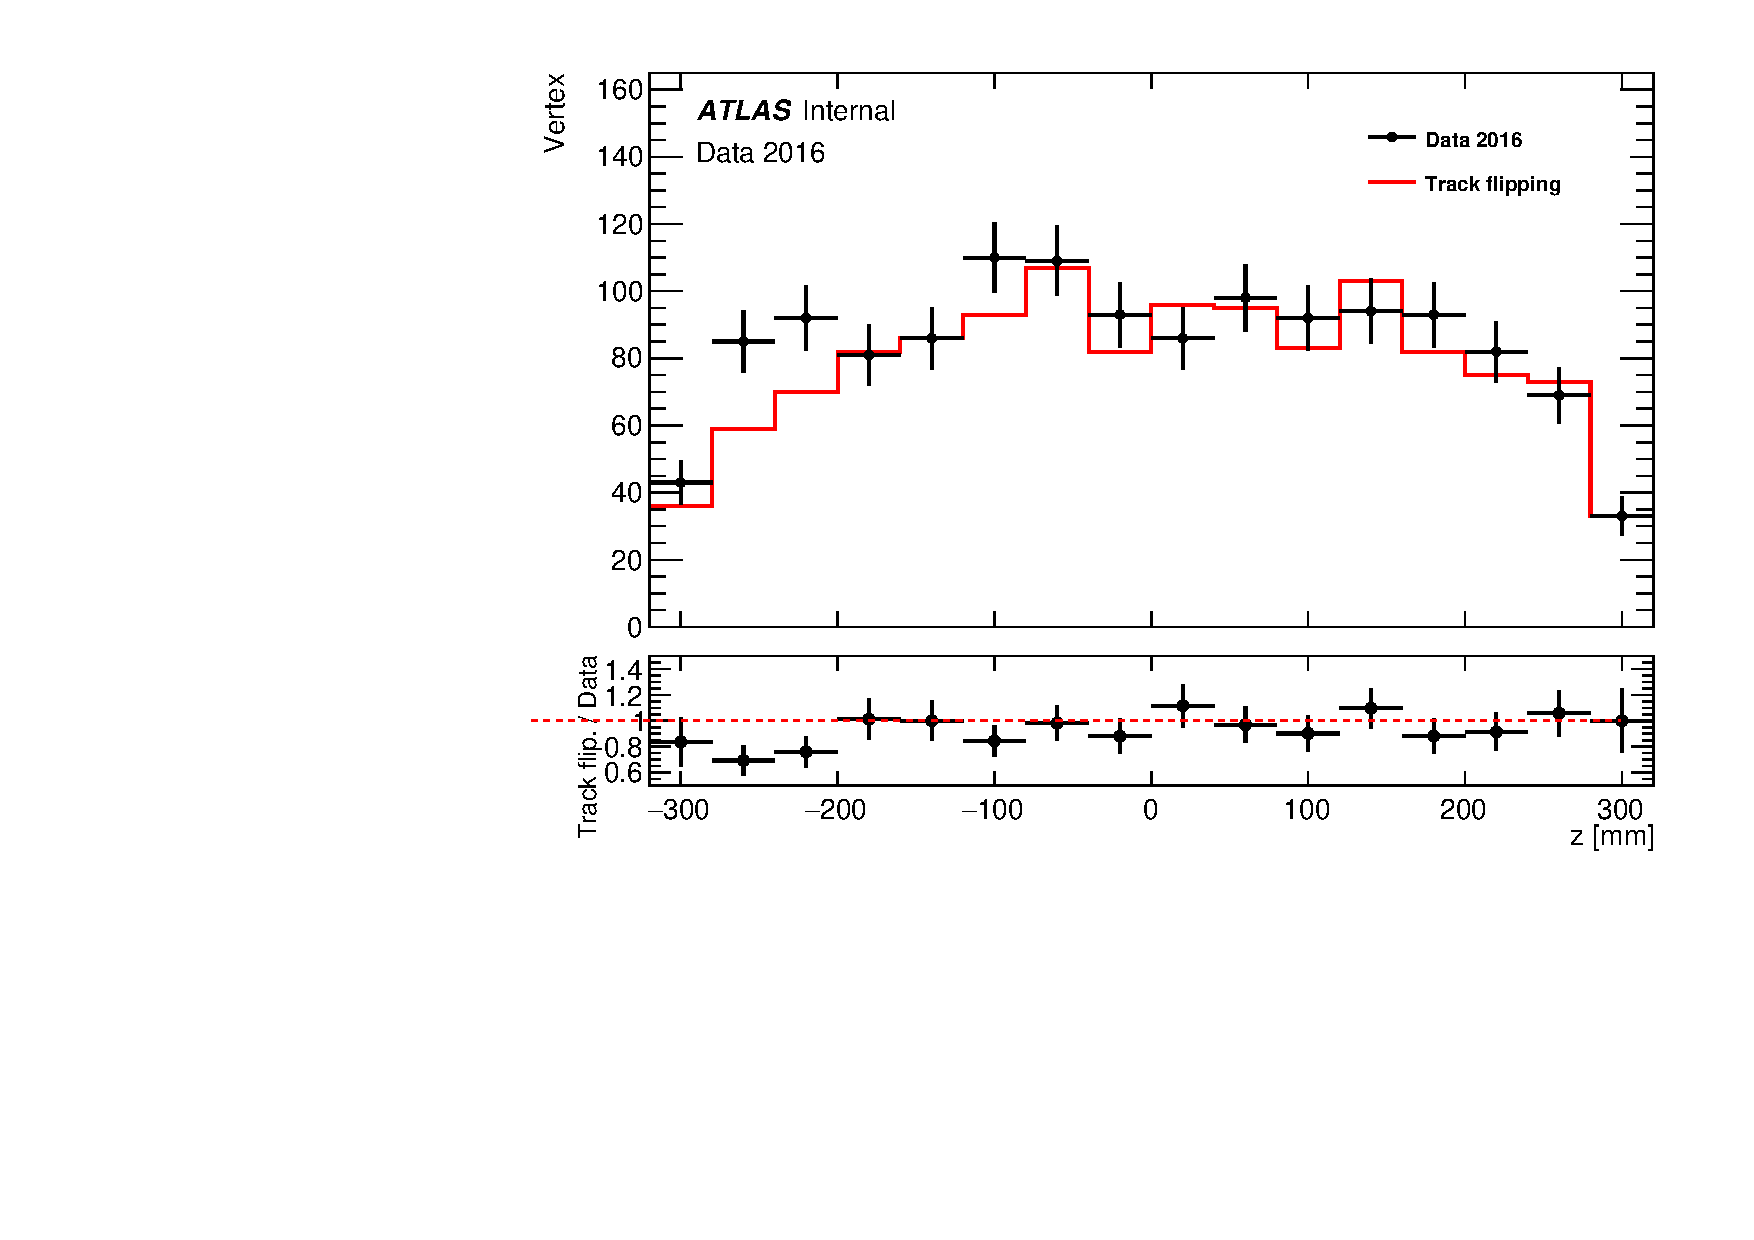
\includegraphics[width=0.45\textwidth]{figures/m_FBE_data_z.pdf}}
    %\subfloat[l]{\label{subfig:random-crossing_l}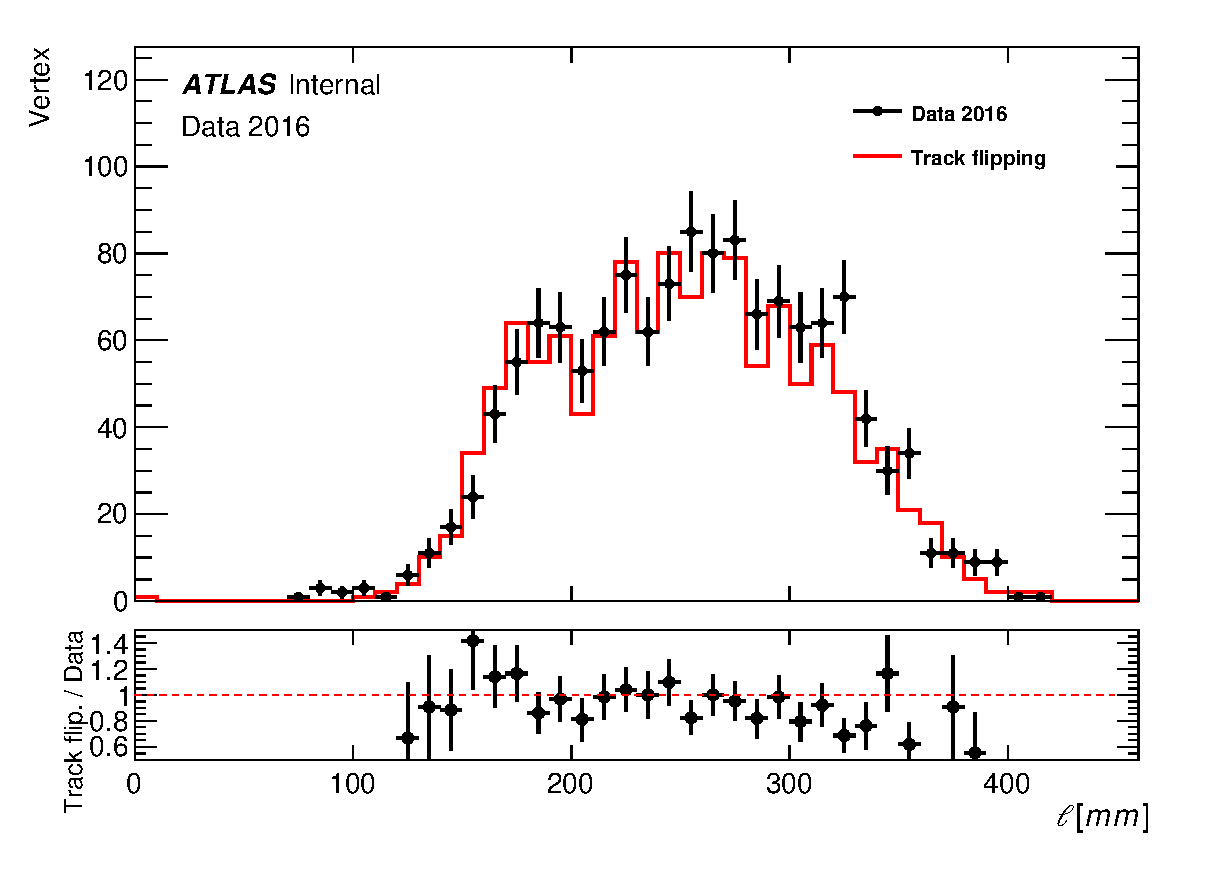
\includegraphics[width=0.45\textwidth]{figures/m_FBE_data_l.eps}}
    \caption{Comparison of (a) vertex mass, (b) $\chi^{2} / \mathrm{DOF}$, (c) transverse, and (d) longitudinal position of vertex found in 32.8 $\mathrm{fb^{-1}}$ of 2016 data sample with those found from the track flipping in the control region of the data sample. In (c), the red dashed lines indicate the four Pixel layers and the first layer of SCT. The green dotted lines indicate the Inner Support Tube (45.5 mm) and Pixel Support Tube (229 mm).}
    \label{fig:random-crossing_vertex_dist_data}
\end{figure}

 Because of the limited statistics in lepton pairs in the data sample, track-flipping vertex yields in the signal region cannot be directly used as random-crossing background estimation. Instead, track-flipping vertex yields in the control region and validation region are extrapolated to estimate random-crossing background in the signal region using lepton probability, defined as follows:
\begin{itemize}
\item $P(e)$ is defined as the ratio of electrons to inner detector tracks in an entire sample,
\item $P(\mu)$ is defined as the ratio of muons to inner detector tracks in an entire sample,
\end{itemize}
where track requirements described in Section~\ref{sec:random_crossing_MC} is required to both leptons and inner detector tracks.

\textbf{Extrapolation from control region} The track-flipping vertex yields in the control region is extrapolated to the signal and validation regions to estimate vertex yields using Eq.~\ref{eq:TF_extrapolation_from_control}. The estimated $\mu x$ and $ex$ vertex yields are compared with the observed track-flipping vertex yield in validation region to calculate scale factors. The scale factor estimated from the extrapolation $xx\rightarrow \mu x$ ($xx\rightarrow ex$) is 0.82 (0.19). The estimated scale factors are applied to the extrapolation to the signal region using Eq.~\ref{eq:TF_scale_factors} to obtain the random-crossing background estimation.

\textbf{Extrapolation from validation region} Similarly, the track-flipping vertex yields in the validation region is extrapolated to the signal to estimate vertex yields using Eq.~\ref{eq:TF_extrapolation_from_validation}. The scale factors are applied to the extrapolation to obtain the background estimation.

The lepton probability, track-flipping and reconstructed vertex yields, scale factors, and estimated random-crossing background are summarized in Table~\ref{table:track_flipping}.

\begin{table}[!htb]%
  \centering
  \subfloat[Lepton probability]{
    \begin{tabular}[t]{ccc}
        \hline\hline
                & Tracks             & P($\ell$)           \\
         \hline
         x      & $2.47\times10^{7}$ & -                   \\
         $\mu$  & $5.23\times10^{4}$ & $2.10\times10^{-3}$ \\
         $e$    & $3.63\times10^{4}$ & $1.46\times10^{-3}$ \\
         Sum    & $2.48\times10^{7}$ & - \\
        \hline\hline
    \end{tabular}
  }%
  \qquad
  \subfloat[Vertex yields]{
    \begin{tabular}[t]{ccc}
        \hline\hline
                & Tracks-flipping    & Data                \\
         \hline
         $xx$   & 1255               & 1346                \\
         $\mu x$& 3                  & 4                   \\
         $ex$   & 1                  & 0                   \\
        \hline\hline
    \end{tabular}
  }%
  \qquad
  \subfloat[Scale factors]{
    \begin{tabular}[t]{cc}
        \hline\hline
         Type                      & SF      \\
         \hline
         $S_{xx\rightarrow\mu x}$  & 0.82              \\
         $S_{xx\rightarrow ex}$    & 0.19              \\
        \hline\hline
    \end{tabular}
  }%

  \subfloat[Extrapolation from control region]{
    \begin{tabular}[t]{ccc}
        \hline\hline
                         & Estimation          & Applying SF         \\
         \hline
         $N_{\mu x}$     & 4                   & -                   \\
         $N_{e x}$       & 5                   & -                   \\
         $N_{\mu\mu}$    & $2.69\times10^{-3}$ & $1.79\times10^{-3}$ \\
         $N_{ee}$        & $5.56\times10^{-3}$ & $1.99\times10^{-4}$ \\
         $N_{e\mu}$      & $7.73\times10^{-3}$ & $1.96\times10^{-3}$ \\
        \hline\hline
    \end{tabular}
  }%
  \qquad
  \subfloat[Extrapolation from validation region]{
    \begin{tabular}[t]{ccc}
        \hline\hline
                         & Estimation          & Applying SF         \\
         \hline
         $N_{\mu\mu}$    & $2.19\times10^{-3}$ & $1.79\times10^{-3}$ \\
         $N_{ee}$        & $1.05\times10^{-3}$ & $1.99\times10^{-4}$ \\
         $N_{e\mu}$      & $3.89\times10^{-3}$ & $1.96\times10^{-3}$ \\
        \hline\hline
    \end{tabular}
  }%
  
  \caption{Random-crossing background by track flipping}%
  \label{table:track_flipping}
\end{table}

\subsubsection{Systematic uncertainty in the track flipping method}
\label{sec:random_crossing_systematics}

The systematic uncertainty in the track flipping method is estimated by studying the variance in background estimation from different variations of the track flipping method. In addition to the transformation described in the previous section ($d_{0}\rightarrow -d_{0}, z_{0}\rightarrow -z_{0}, \phi\rightarrow\phi-\pi, \theta\rightarrow\pi-\theta$), the following track transformations are considered.
\begin{itemize}
\item \textbf{Same sign d0}: $d_{0}\rightarrow d_{0}, z_{0}\rightarrow -z_{0}, \phi\rightarrow\phi-\pi, \theta\rightarrow\pi-\theta$
\item \textbf{Same sign $\theta$}: $d_{0}\rightarrow -d_{0}, z_{0}\rightarrow -z_{0}, \phi\rightarrow\phi-\pi, \theta\rightarrow\theta$
\item \textbf{90 degrees rotation in $\phi$}: $d_{0}\rightarrow -d_{0}, z_{0}\rightarrow -z_{0}, \phi\rightarrow\phi-\frac{\pi}{2}, \theta\rightarrow\theta$
\end{itemize}


\textbf{NEED TO ADD RESULTS HERE}

\newpage






\subsection{Cosmic background}
\label{sec:cosmic_ray}
Cosmic background is the dominant source of backgrounds in $\mu\mu$ channel as a cosmic muon can be reconstructed as a back-to-back $\mu\mu$ vertex with large displacement from the primary vertex. Cosmic veto is introduced to suppress the background from such vertices by requiring $R_{\mathrm{CR}} = \sqrt{(\Delta \phi - \pi)^{2} + (\Sigma \eta)^{2}} >$ 0.04 where $\Delta \phi$, $\Sigma \eta$ are the difference and sum of track parameters from two tracks at a vertex, respectively. For a back-to-back vertex, $R_{\mathrm{CR}}$ is expected to be close to 0. The vertex cut flow in Figure~\ref{fig:signal_cutflow_MC_mumu} shows that the efficiency loss due to the cosmic veto is negligible.

In order to estimate the cosmic background, \textit{cosmic control region} is defined by inverting the cosmic veto cut (i.e. $R_{CR} < 0.04$). All other event and vertex selections are kept the same as the signal region. Figure~\ref{subfig:cosmic_cutflow} shows the vertex cut flow of the cosmic control region in the data sample. There are 127 $\mu\mu$ vertices found with $R_{CR} < 0.04$, and no $ee$ or $e\mu$ vertex was found. Figure~\ref{subfig:cosmic_Rcr} shows the $R_{CR}$ distribution of these vertices. All vertices found in the cosmic control region have very small $R_{CR}$. The $R_{CR}$ distribution is fitted with gaussian function and then extrapolated into the signal region, and the cosmic background is estimated to be negligible.


%and the extrapolation of the fit estimates that the cosmic background in the signal region is less than $10^{-19}$.
% Pairs of muon tracks found in data that satisfies $R_{CR} < 0.04$ are shown as an upper bound of $\mu\mu$ vertex yields.
%The exponential distribution suggests that no cosmic muon background is expected in the signal region.

%The extrapolation of the exponential fit to $R_{CR}$ distribution of $\mu\mu$ vertex estimates that the cosmic muon background in the signal region is less than $10^{-19}$.


\begin{figure}[!htb]
    \centering
    \subfloat[]{\label{subfig:cosmic_cutflow}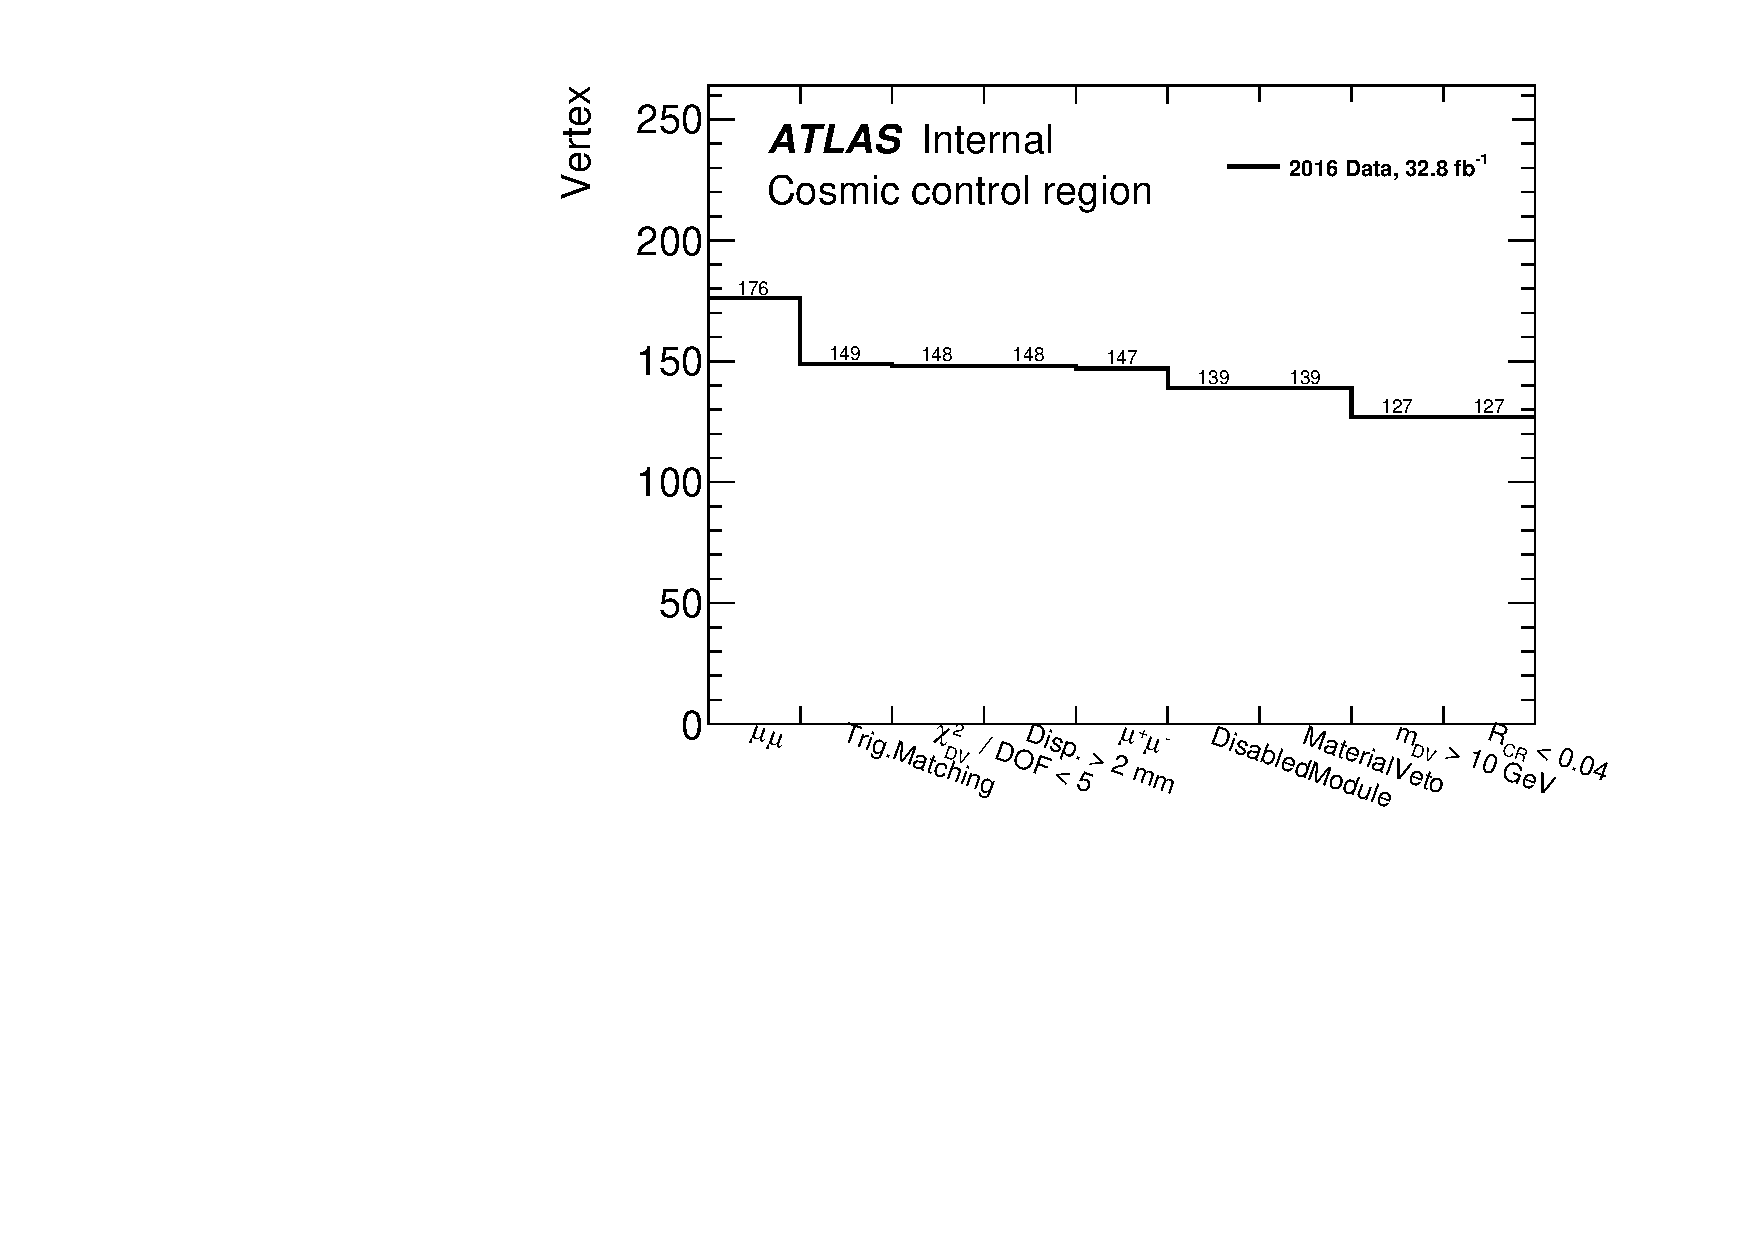
\includegraphics[width=0.50\textwidth]{figures/m_data_cosmic_vertex_cutflow_mumu.pdf}}
    \subfloat[]{\label{subfig:cosmic_Rcr}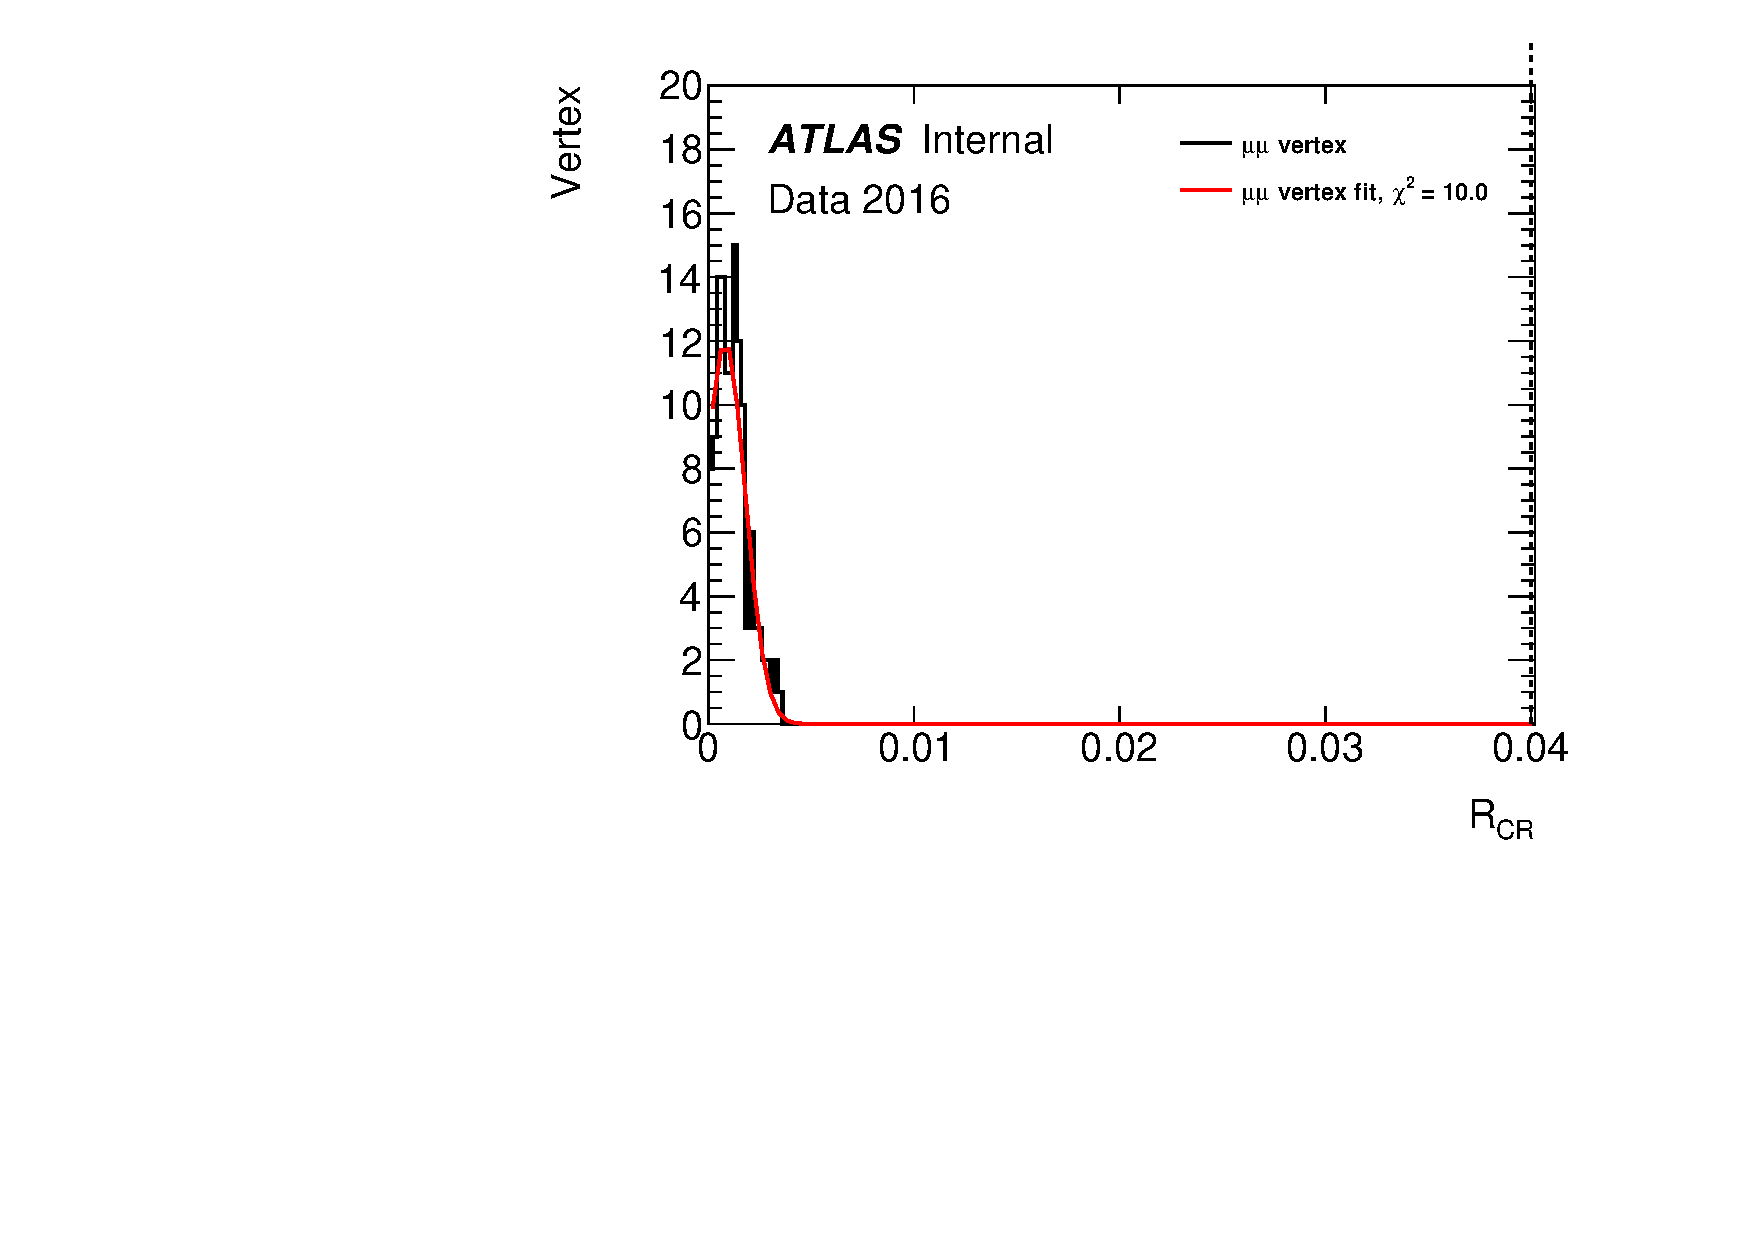
\includegraphics[width=0.50\textwidth]{figures/m_cosmic_background.pdf}}
    \caption{(a) Vertex cut flow of the cosmic control region, and (b) $R_{CR}$ distribution of $\mu\mu$ vertex found in the data sample. The curve shows a fit with an exponential function.}
    \label{fig:cosmic_control}
\end{figure}


\subsection{Low-mass background}
\label{sec:low_mass}
A SM process such as photon conversion or the decay of a low-mass particle, e.g. $J/\psi$, can be reconstructed as a low-mass, displaced vertex decaying to a dilepton final state. Low-mass veto is implemented to suppress background from these displaced vertices ($m > 10$ GeV). Due to large mass of $Z'$ in the signal MC samples, there is no efficiency loss by the veto.

\textit{Low-mass control region} is used to estimate the low-mass background by inverting the low-mass cut (i.e. $m < 10$ GeV). All other event and vertex selections are kept the same as the signal region. 

Figure~\ref{fig:lowmass_control} shows the vertex cut flow and mass distribution of the vertices found in the low-mass control region in the data. There are 12 vertices with $m < $ 10 GeV, passing all other signal selections. The mass spectrum is fitted with the sum of a Gaussian centered around $3$ GeV, representing $J/\psi$ resonance, and an exponential for the background distribution. The extrapolation of the combined fit yields an estimate of $\backsim 0.09$ vertices in the signal region.
%The $R_{CR}$ distribution of $\mu\mu$ vertex is fitted with an exponential, extrapolated into the signal region yielding an estimate of $10^{-19}$ vertices.



\begin{figure}[!htb]
    \centering
    \subfloat[]{\label{subfig:lowmass_cutflow}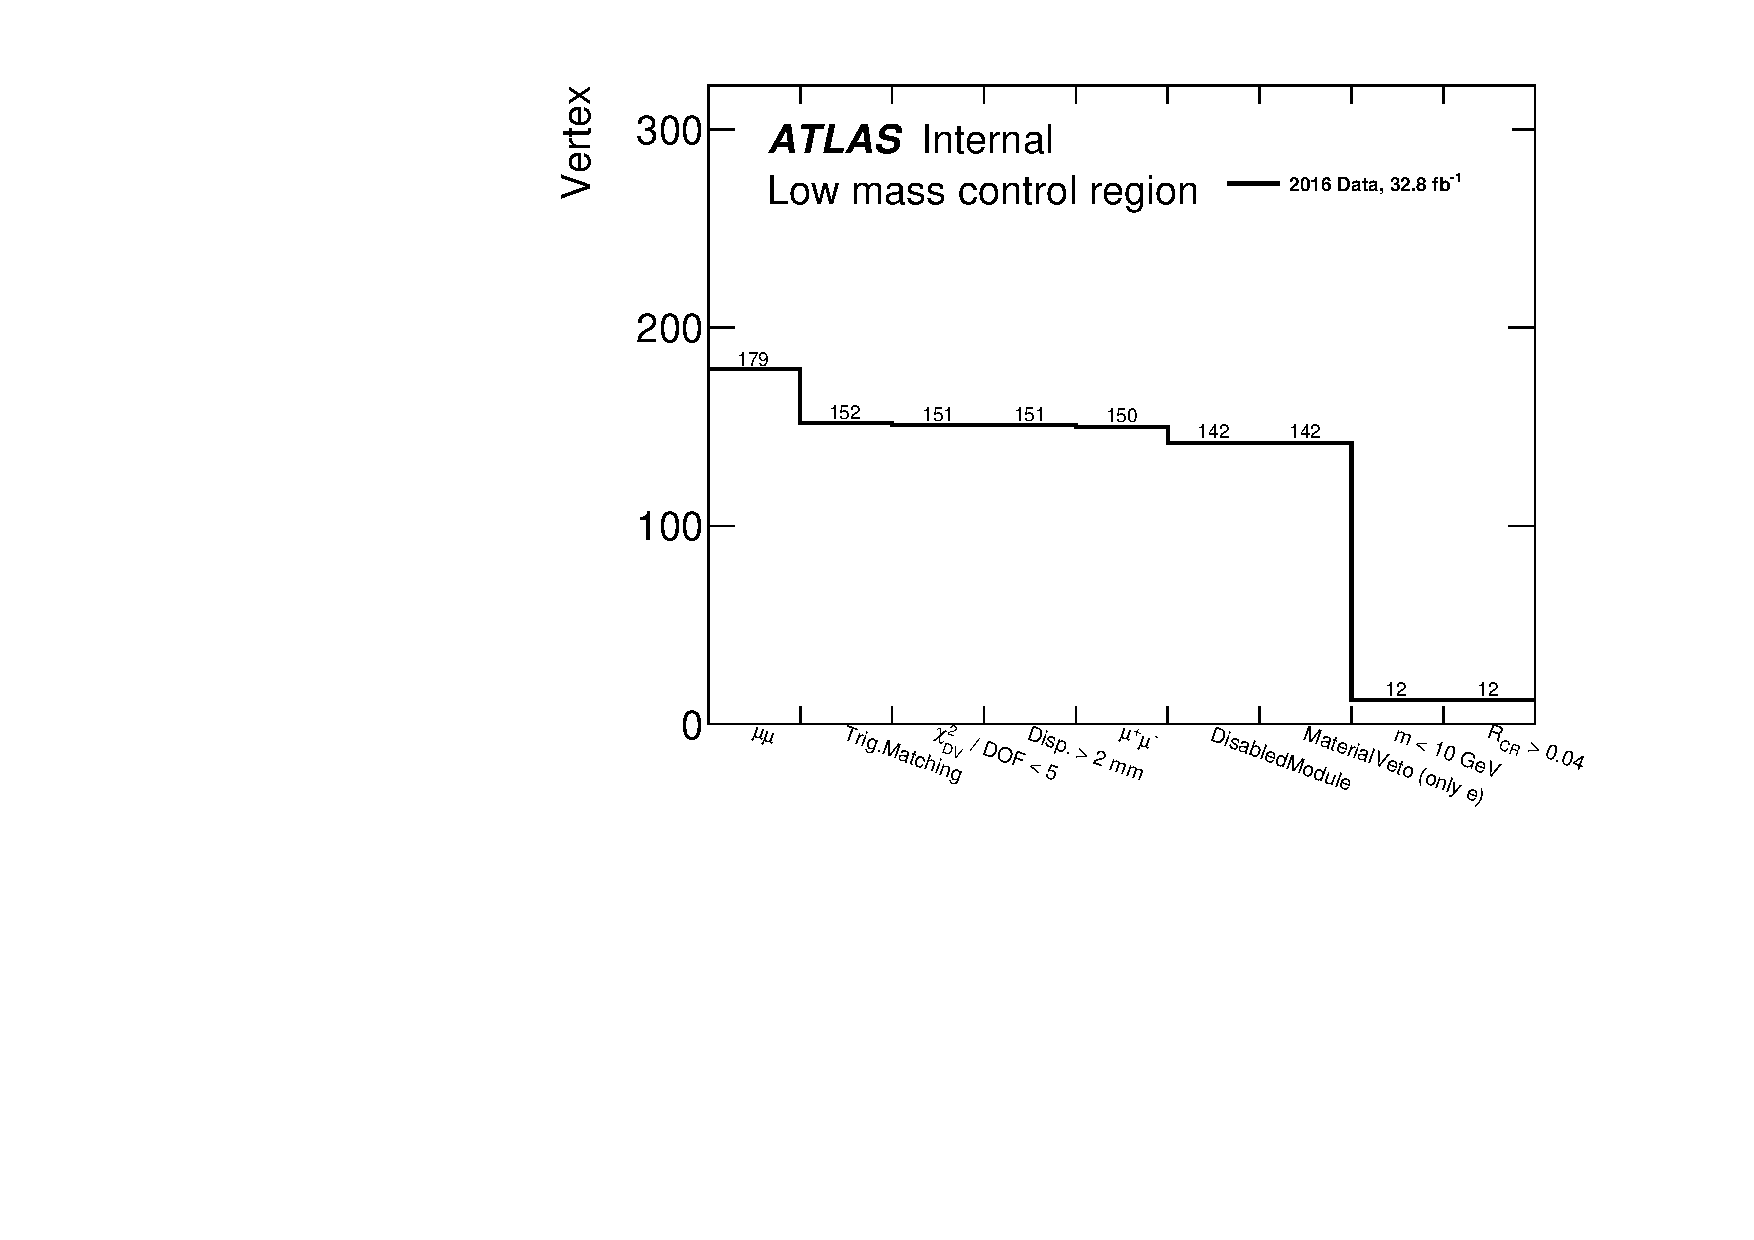
\includegraphics[width=0.50\textwidth]{figures/m_data_dv_cutflow_lowmass_mumu.pdf}}
    \subfloat[]{\label{subfig:lowmass_dist}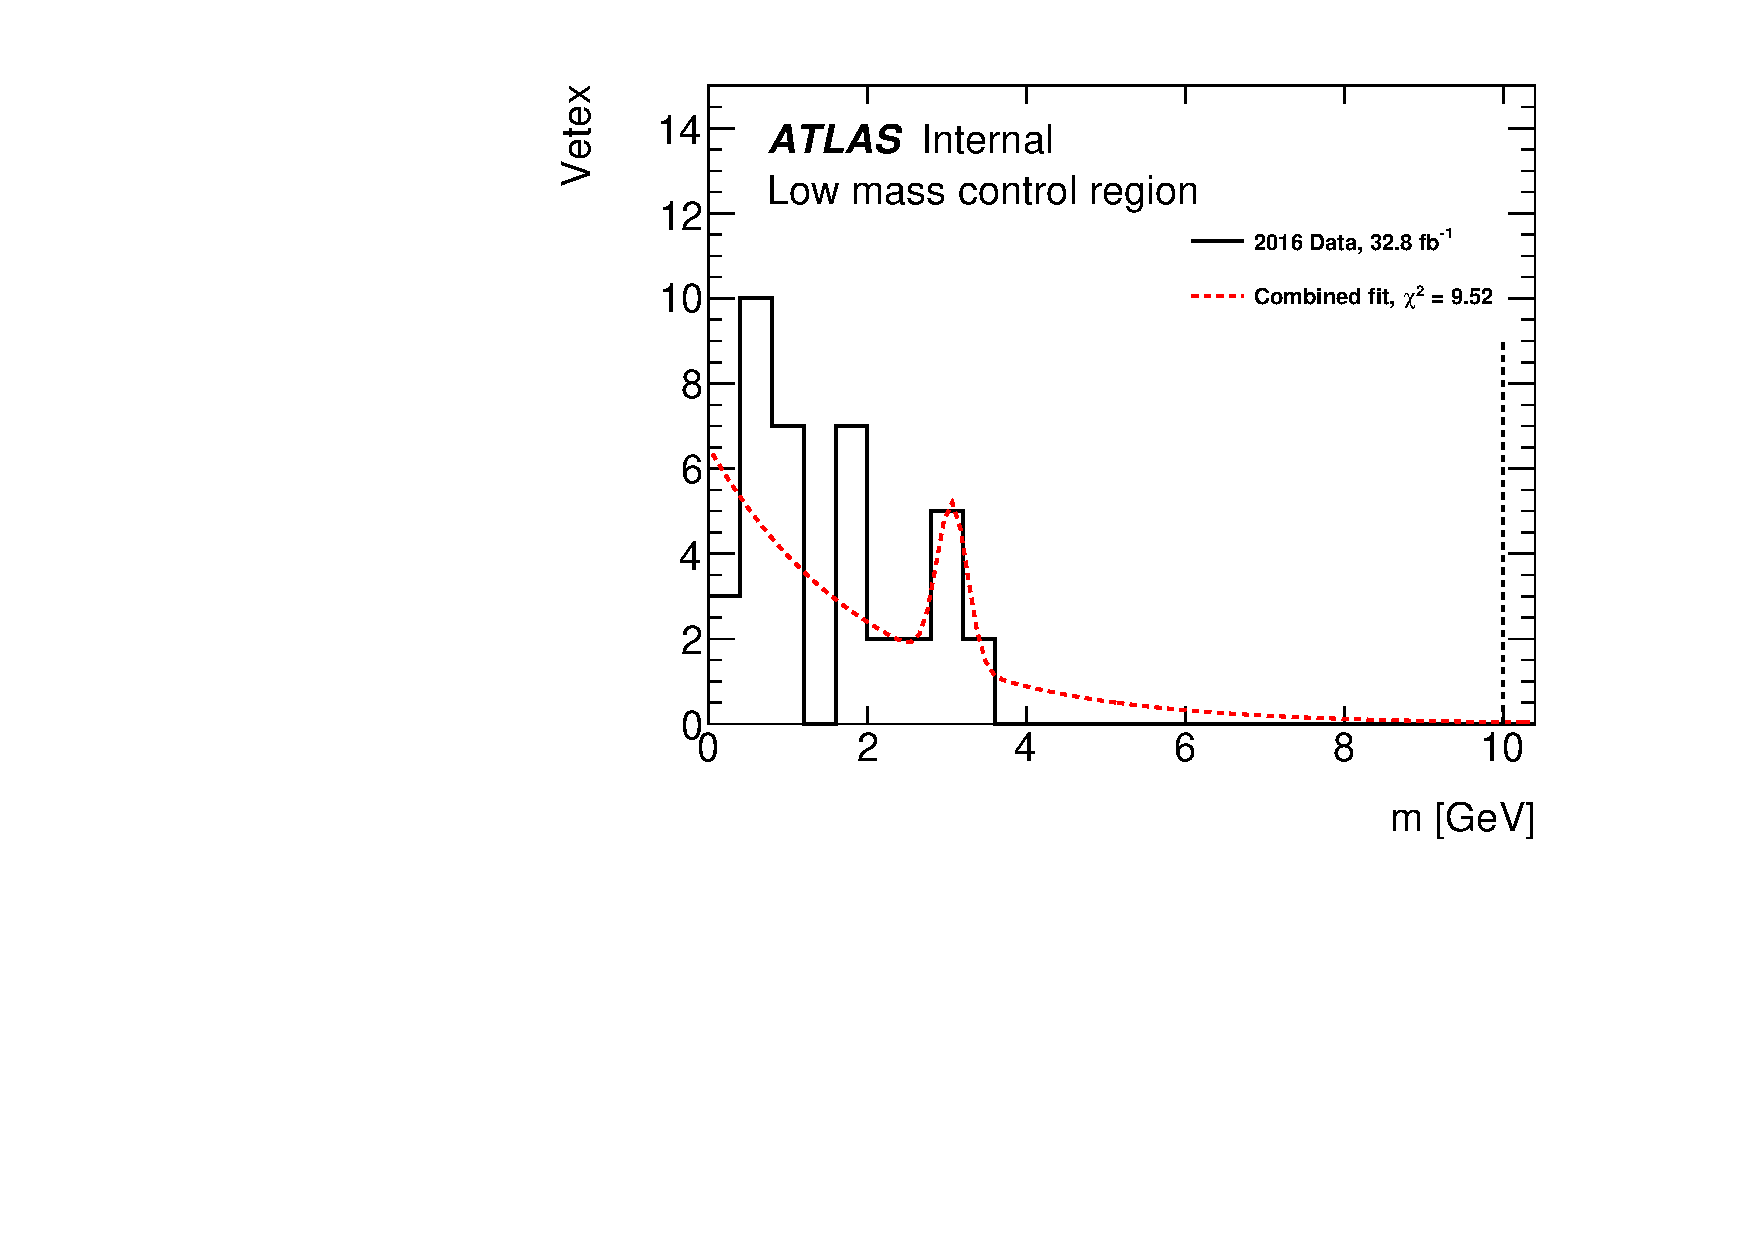
\includegraphics[width=0.50\textwidth]{figures/m_data_dv_mumu_M_low.pdf}}
    \caption{(a) Vertex cut flow and (b) mass distribution of the low-mass control region from the data sample. The combined fit of a Gaussian centered around $3$ GeV, representing $J/\psi$ resonance, and an exponential for the background is used to estimate the low-mass background in the signal region.}
    \label{fig:lowmass_control}
\end{figure}



